% 
%  chapter5.tex
%
\chapter{Implementation}\label{ch:impl}

This chapter presents the solution developed to create CASCIFFO given the functional requirements detailed previously. It describes the techniques used and choices made throughout the implementation of the solution.

It is structured with the following sections:
\begin{itemize}
    \item Back-end~\ref{ch:impl:sec:be}: Describes the back-end module.
    \item Front-end~\ref{ch:impl:sec:fe}: Describes the front-end module.
    \item Heroku deployment~\ref{ch:impl:sec:install-deploy:ss:heroku}: Usage of cloud-based platform Heroku for continuous development.
    \item On-Premises Deployement~\ref{ch:impl:sec:install-deploy:ss:on-premises}: Deploying the application on-premises hosted by Apache.
\end{itemize}


\section{Back-end module}\label{ch:impl:sec:be}
This section describes the implementation choices and details of the Back-end module.
It first introduces the development of the back-end module and follows into more details regarding the repositories, services, controllers, mappers and authentication respectively.

This section is structured as follows:
\begin{itemize}
    \item Framework Stack~\ref{ch:impl:sec:be:subsec:be-module-dev} - Describes the technology used to created the framework stack of the \acrshort{be} module;
    \item PostgreSQL database~\ref{ch:impl:sec:be:subsec:config-postgresql} - Explains the configuration a creation of the PostgreSQL database used;
    \item Initial Development~\ref{ch:impl:sec:be:subsec:be-init-dev} - Describes in detail the steps initially taken for the implementation of the back-end module;
    \item Spring Configuration~\ref{ch:impl:sec:be:subsec:be-spring-config} - Details the Spring configuration to allow the module to run as expected;
    \item Repositories~\ref{ch:impl:sec:be:subsec:repositories} - Explains and details how the repositories function and their creation;
    \item Services~\ref{ch:impl:sec:be:subsec:services} - Details the functionality of the services in the module and shows three examples of services used in the implementation;
    \item Controllers~\ref{ch:impl:sec:be:subsec:controllers} - Describes how controllers work and their role in the module;
    \item Mappers~\ref{ch:impl:sec:be:subsec:mappers} - Details how the role of mappers in the module, how they are used and how we can take advantage of Spring features to make a sustainable and maintainable codebase;
    \item Authentication~\ref{ch:impl:sec:be:subsec:authentication} - Describes how the authentication works and it's implemented;
    \item Exception Handling~\ref{ch:impl:sec:be:subsec:exceptions} - Describes the steps taken to raise and handle exceptions.
\end{itemize}


\subsection{Framework Stack}\label{ch:impl:sec:be:subsec:be-module-dev}

The back-end module was developed using \textit{Spring Webflux}~\cite{spring-webflux} over Spring Web due to the reactive nature. \textit{Spring Webflux}~\cite{spring-webflux} brings a fully non-blocking programming environment and provides asynchronous calls to the database through the \textit{R2DBC} driver. This allows for a completely non-blocking experience from the moment an HTTP request is received. 

The module consists of three layers, the Repository layer, which is responsible for database access, the Service layer, which is responsible for business logic, and finally the Controller layer, which receives and responds to requests. The layers communicate only with the layers below them, preventing circular dependencies. The controller layer communicates with the service layer, the service layer communicates with the repository layer and the latter communicates directly with the database. Across these layers there are exception handlers to handle any foreseen and unforeseen exceptions.


\subsection{PostgreSQL database}\label{ch:impl:sec:be:subsec:config-postgresql}

Following the detailed data model described in~\ref{ch:architecture:sec:data-model}, a SQL script, written in PostgreSQL language was created to entail the creation of the database, the user ownership and initial data of the database. The script is over 2 thousand lines long, thus not available as an appendix, however, it is available on the Github Repository Casciffo\footnote{\url{https://github.com/ValdemarPCAntunes/casciffo}}~\label{fn:gh-casciffo-impl} along with the rest of the essentials to run the platform locally.

The only configuration required is the existence of a user \lstinline{vp} who's credentials are be used in the Spring configuration explained further on.  


\subsection{Initial Development}\label{ch:impl:sec:be:subsec:be-init-dev}

By using the tool \textit{Spring Initializr}~\footnote{\url{https://start.spring.io/}}\label{fn:spring-io} provided by \textit{Spring} we're able to start with a project containing the necessary dependencies ready to launch. The project type was chosen to be Gradle-Kotlin, developed in Kotlin language, as illustrated in figure~\ref{fig:spring-io-start}.

\begin{figure}[H]
    \centering
    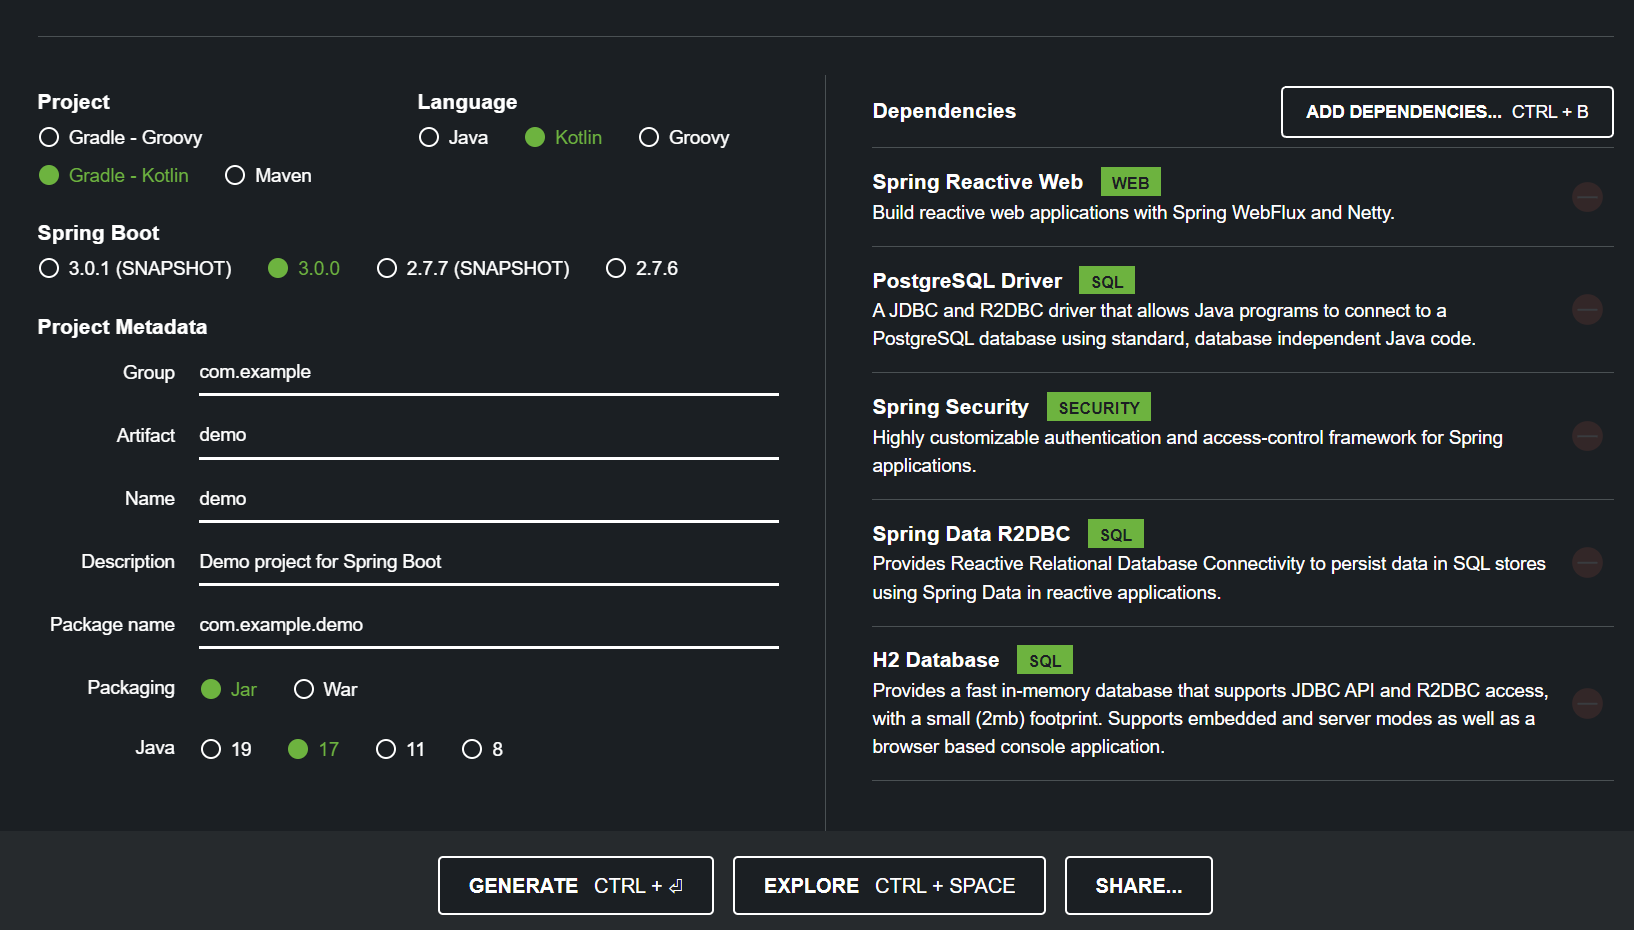
\includegraphics[scale=0.35]{Chapters/img/misc/spring-io.png}
    \caption{Initial project structure using \textit{Spring Initializr}.}
    \label{fig:spring-io-start}
\end{figure}

After downloading the project template, the project was organized by folders corresponding to each entity, this was chosen for the convenience of navigation due to the amount of entities.

In each entity folder, a class representing the controller, service and repository layer was created alongside the entity model itself.

The next step in development was the configuration of the spring application.

\subsection{Spring Configuration}~\label{ch:impl:sec:be:subsec:be-spring-config}
Given the starting project we first need to set the database credentials so that Spring knows how handle database access requests. This was achieved by utilizing the file \lstinline{application.properties} inside the resources folder, in the case it doesn't exist, create it. The properties: \lstinline{spring.r2dbc.url} - refers to the full URL of the database location, in the following format \lstinline[keywordstyle=\color{black},commentstyle=\color{black},stringstyle=\color{black}]{r2dbc:postgresql://[HOST]:[PORT]/[DATABASE_NAME]}, in the exceptional case that the PostgreSQL service runs on a different port from the default 5432, the attribute PORT in the mentioned format should be changed accordingly; \lstinline{spring.r2dbc.username} and \lstinline{spring.r2dbc.password} correspond to the database credentials used for each connection made during a database access operation. Other fields can be set to make use of the potential Spring offers, such as:
\begin{itemize}
    \item \lstinline{spring.jackson.locale} --- Serves to indicate what type of \textit{JSON} serialization to use, the locale that should be considered for formatting dates, the used value was \lstinline{pt_PT};
    
    \item \lstinline[keywordstyle=\color{black},commentstyle=\color{black},stringstyle=\color{black}]{spring.jackson.default-property-inclusion} --- Setting this property to \lstinline[keywordstyle=\color{black},commentstyle=\color{black},stringstyle=\color{black}]{non_null} indicates that Spring's serializer that only properties with non-null values are to be included in REST requests and responses.
    
    \item \lstinline{server.port} --- Sets the port on which the Spring application will be started on, defaults to 8080.
    
    \item \lstinline{server.error.include-message} --- Indicates whether an error message should be attached to an error response, defaults to \lstinline{never} to possibly prevent sensitive information leaking, in the context of CASCIFFO, this wasn't a worry so it was set to \lstinline{always} as a way to not only debug but also better handle exceptions in the \acrshort{fe}.
    
    \item \lstinline{spring.web.resources.static-locations} --- Indicates the location of static resources to be served by Spring. This property is crucial to the development and deployment of the application, as the static resources consist of the optimized \acrshort{fe} module production build. 
    
    It was set with \lstinline{file:./webapp}, the prefix \lstinline{file:} serves to point out to Spring that the following argument corresponds to a file path. In this specific case, the prefixed dot in \lstinline{./webapp} corresponds to the relative path from the directory that the app was started in. 
    
    \item \lstinline{spring.r2dbc.properties.sslMode} --- This property defines whether the connection to the database requires SSL mode to successfully establish a connection. During continuous development with the platform \textit{Heroku} this setting was set to \lstinline{REQUIRE}, since the database was hosted via HTTPS. During deployment and local development this property was commented out. 
\end{itemize}   

Another type of properties which are substantially helpful during development are the logging options, prefixed with \lstinline[keywordstyle=\color{black},commentstyle=\color{black},stringstyle=\color{black}]{logging.level}. 
By default they have the value of \lstinline{INFO}, and by changing them to \lstinline{DEBUG} the information displayed during run-time reflects the execution of each operation in a very transparent manner which was most useful for testing purposes. 
During development the value of the properties \lstinline[keywordstyle=\color{black},commentstyle=\color{black},stringstyle=\color{black}]{logging.level.web} - which refers to incoming and outgoing requests; \lstinline[keywordstyle=\color{black},commentstyle=\color{black},stringstyle=\color{black}]{logging.level.org.springframework.security} - which refers to security web filters and finally \lstinline[keywordstyle=\color{black},commentstyle=\color{black},stringstyle=\color{black}]{logging.level.org.springframework.r2dbc} - which refers to the database queries being executed. 

To compile and execute the spring application without an integrated development environment (IDE) like IntelliJ we can use the files present inside the project directory, namely the file~\lstinline{gradlew} and \lstinline{build.gradle.kts}. The former executes \textit{gradle tasks} while the latter is where we configure said tasks and explicitly state the dependencies of the project. 
To compile the project we can run a terminal like using ~\lstinline{gradlew build -x test} which will compile and bundle the project sources into a \textit{JAR} file which we can later execute using \textit{Java} commands. The specification \lstinline{-x test} is useful for a production build since it tells Gradle to skip the tests task.

The dependencies required for the implementation of this module are present in the listing~\ref{lst:gradle-config}. This configuration snippet includes the dependencies for \textit{Spring Security}, \textit{Spring Webflux} and \textit{Kotlin coroutines}, all of which will be mentioned further on this document.

\begin{lstlisting}[
caption={Gradle configurations for production build.},
label={lst:gradle-config}
]

plugins {
	id("org.springframework.boot") version "2.6.3" //Spring boot
	id("io.spring.dependency-management") version "1.0.11.RELEASE" 
	kotlin("jvm") version "1.6.10" //Kotlin jvm
	kotlin("plugin.spring") version "1.6.10" //Support for spring boot in a kotlin project 
}

dependencies {
implementation("org.springframework.boot:spring-boot-starter-security") //Spring Security
implementation("org.springframework.boot:spring-boot-starter-data-r2dbc:3.0.0") //Spring Data R2DBC
implementation("org.springframework.boot:spring-boot-starter-webflux") //Spring Webflux
implementation("io.projectreactor.kotlin:reactor-kotlin-extensions:1.1.7") //Kotlin Flow
implementation("org.jetbrains.kotlinx:kotlinx-coroutines-reactor:1.6.4") //Kotlin coroutines
implementation("org.jetbrains.kotlin:kotlin-reflect") //Kotlin reflection
implementation("org.jetbrains.kotlin:kotlin-stdlib-jdk8")

//PostgreSQL
runtimeOnly("io.r2dbc:r2dbc-postgresql:0.8.13.RELEASE")
runtimeOnly("org.postgresql:postgresql:42.5.1")

//Json Web Tokens
implementation("io.jsonwebtoken:jjwt-api:0.11.5")
runtimeOnly("io.jsonwebtoken:jjwt-impl:0.11.5")
runtimeOnly("io.jsonwebtoken:jjwt-jackson:0.11.5")
}
\end{lstlisting}

From this snippet we can observe the keywords \lstinline{runtimeOnly} and \lstinline{implementation}, these keywords refer as to when the libraries are required, as the name implies, the former keyword means that the library will only be included during run-time whereas the \lstinline{implementation} dependencies are required for the implementation, compilation of the project and subsequently run-time as well.
This helps to keep the compile \textit{classpath} smaller and faster.

The \lstinline{plugins} property is used to specified the plugins required to run the project. A plugin is a set of tasks and configurations that can be added to a project to extend its functionality, in this case we require the plugins related to \textit{Spring} and \textit{Kotlin}.


\subsection{Repositories}\label{ch:impl:sec:be:subsec:repositories}

The repository layer is responsible for directly accessing and manipulating data in the database. 


The repositories are interfaces annotated with Spring's \lstinline{@Repository}, indicating they behave as a repository, each repository should implement an appropriate public interface, in the reactive context, it can either be \lstinline{ReactiveCrudRepository} or \lstinline{ReactiveSortingRepository} followed by the type of entity and type of identifier (such as \lstinline{ReactiveCrudRepository<Entity, EntityIdType}), where the former allows for basic CRUD operations (Create, Read, Update, Delete) without needing to implement further functionality, while the latter allows for built-in sorting functionalities. Spring also allows custom functions to be implemented either through naming conventions, such as \lstinline{findAllByIdAndFieldIs(id, field)}, and through custom queries. For more complex queries another option is available, by annotating a method with \lstinline{@Query(sql: String)} and passing a \lstinline{string} argument with the SQL statement defined at design time. All repository methods return a type encapsulated by either \lstinline{Mono} or \lstinline{Flux}. The type \lstinline{Mono} should be returned when the method is expected to return between zero and a single result, while \lstinline{Flux} should be used a result varying between zero and $n$ elements are expected. These features can be seen in the listing~\ref{lst:proposal-repo-class} below.

\begin{lstlisting}[
label={lst:proposal-repo-class},
language={kt},
caption={Repository used for the Proposal entity.}]
@Repository
interface ProposalRepository : ReactiveSortingRepository<ProposalModel, Int> {

    @Query(
        "SELECT COUNT(*) " +
                "FROM proposal p " +
                "WHERE p.proposal_type = :type"
    )
    fun getCountByType(type: ResearchType): Mono<Int>

    @Query(
        "SELECT COUNT(*) filter ( where p.proposal_type = 'OBSERVATIONAL_STUDY' ) as studies, " +
        "COUNT(*) filter ( where p.proposal_type = 'CLINICAL_TRIAL' ) as trials " +
        "FROM proposal p"
    )
    fun countTypes(): Mono<CountHolder>
    
    fun findAllBySiglaLike(sigla: String): Flux<ProposalModel>

}    
\end{lstlisting}

A key factor to let the~\textit{Spring Webflux}~\cite{spring-webflux} framework know a data class is an entity, for the main purposes of saving and updating, is annotating said class with \lstinline[keywordstyle=\color{black},commentstyle=\color{black},stringstyle=\color{black}]{@Table("table_name")} where \lstinline[keywordstyle=\color{black},commentstyle=\color{black},stringstyle=\color{black}]{"table_name"} refers directly to the database table, and the identifier field with \lstinline{@Id} which also directly corresponds to the identifier present in the mentioned table. It is worth noting that the identifier of a database table must be numeric. As briefly mentioned in \cref{ch:architecture:sec:data-model}, text identifiers and compound keys don't function properly with this framework, in order to circumvent this, each database table has its own unique numeric identifier. 

When creating an entity, the property annotated with \lstinline{@Id} must a value of \lstinline[keywordstyle=\color{black},commentstyle=\color{black},stringstyle=\color{black}]{null}, otherwise, the framework will attempt to update an nonexistent entity. To work around this, we can either implement a custom repository and override the \lstinline{save()} method or design the entities used to have an automatically generated identifier. The approach taken while building CASCIFFO's data model was the latter.

It should also be noted that naming conventions are taken into account between the database and the entity, the \textit{Snake Case} naming convention used by \textit{PostgreSQL}, is automatically converted into \textit{Camel Case} in \textit{Spring}, for example a table field named \lstinline[keywordstyle=\color{black},commentstyle=\color{black},stringstyle=\color{black}]{created_date} is automatically converted into \lstinline{createdDate}. 
This automation is very useful when the mapped object contains the property \lstinline{createdDate}, however, what if the property was named \lstinline{createdOn}?

In such cases, two different approaches can be used to answer this question. Firstly we can customize the repository fetch method by including the annotation \lstinline[keywordstyle=\color{black},commentstyle=\color{black},stringstyle=\color{black}]{@Query("sql_statement"} followed up with writing a select that renames \lstinline[keywordstyle=\color{black},commentstyle=\color{black},stringstyle=\color{black}]{created_date} to \lstinline[keywordstyle=\color{black},commentstyle=\color{black},stringstyle=\color{black}]{created_on}, this takes advantage of the auto naming conversion but requires effort to customize the query. The other approach that was heavily relied on what annotating the property with 
\lstinline[keywordstyle=\color{black},commentstyle=\color{black},stringstyle=\color{black}]{@Column("entity_column")} which indicates what column Spring should map to the property.

By taking the second option, the property \lstinline{createdOn} will be annotated with \lstinline[keywordstyle=\color{black},commentstyle=\color{black},stringstyle=\color{black}]{@Column("created_date")}.


One noticeable downside of using~\textit{Spring Webflux}~\cite{spring-webflux} and R2DBC, is that its current version doesn't provide mechanism of designing complex relationships with annotations, a feature available in \textit{Spring Web}. For example given two entities, A and B, with a relationship of 1-to-1, when fetching entity B, there isn't an automatic mechanism to build the associated entity A, after the fetch, the data will come as-is in the database, as opposed to \textit{Spring Data JPA} where such relationships can be modeled and built by the \textit{Spring Framework}. 
While nested entities can exist in a data class representing a database table, since they can't be loaded through automatic means, they must be annotated with \lstinline{@Transient} alongside \lstinline{@Value(defaultValue)}. 
The former annotation tells \textit{Spring}'s framework to ignore the annotated property when saving a new entity while the latter annotation comes into play during the mapping after a fetch, this annotation defines the default value to assign to the annotated property, in the development context, the value assigned was always \lstinline[keywordstyle=\color{black},commentstyle=\color{black},stringstyle=\color{black}]{@Value("null")}. 

This means that for complex entities with multiple foreign keys, with each foreign key corresponding to a nested object that needs to be manually instantiated, in order to fetch the data to build these objects would require to make that as database calls as there are nested entities which leads to performance issues. To counter this, entities were created to serve as containers of data, by aggregating all the fields required to build not only the base entity but also the nested ones. 
In conjunction with this, for each of these containers a repository was created, however, since the data that we want is split between tables, a custom query is needed to fetch the desired results. By using this approach we can specify all the necessary data manually. To illustrate this, the listing~\ref{lst:proposal-aggregate-fetch} shows a selection of fields from several different database entities, which are then mapped to the aggregate of type \lstinline{ProposalAggregate}. The container of this aggregation doesn't need to be annotated with \lstinline{@Table()} or have \lstinline{@Id} on one of its fields, since it will be exclusively used for fetching data.

\begin{lstlisting}[
label={lst:proposal-aggregate-fetch},
language={kt},
caption={A proposal aggregate repository function that fetches data from multiple sources.}]
@Query(
    "SELECT p.proposal_id, p.sigla, p.created_date, p.last_modified, p.proposal_type, " +
            "pfc.proposal_financial_id, pfc.financial_contract_id, pfc.promoter_id, pfc.has_partnerships, " +
            "state.state_name, st.service_name, pl.pathology_name, ta.therapeutic_area_name, " +
            "promoter_name, user_name " +
    "FROM proposal p " +
    "JOIN states state ON p.state_id = state.state_id " +
    "JOIN pathology pl ON p.pathology_id = pl.pathology_id " +
    "JOIN service st ON st.service_id = p.service_id " +
    "JOIN therapeutic_area ta ON ta.therapeutic_area_id = p.therapeutic_area_id " +
    "JOIN user_account pinv ON p.principal_investigator_id = pinv.user_id " +
    "LEFT JOIN proposal_financial_component pfc ON p.proposal_id = pfc.proposal_id " +
    "LEFT JOIN promoter pr ON pr.promoter_id = pfc.promoter_id " +
    "ORDER BY p.last_modified DESC " +
    "LIMIT :n"
)
fun findLastModifiedProposals(n: Int): Flux<ProposalAggregate>
\end{lstlisting}

The entities associated to each repository are classes which only contain data, as such, \textit{Data classes}, available in Kotlin. 
The data classes were created using the described annotations and followed the mentioned rules. Below is the listing of the proposal data class (\ref{lst:proposal-data-class}) which includes everything mentioned in regards to entities.

\begin{lstlisting}[
label={lst:proposal-data-class},
language={kt},
caption={Data class representing the entity Proposal.}]
@Table(value = "proposal")
data class ProposalModel(
    @Id
    @Column(value = "proposal_id")
    var id: Int? = null,
    @Column(value = "sigla")
    var sigla: String? = null,
    @Column(value = "proposal_type")
    var type: ResearchType? = null,
    @Column(value = "created_date")
    var createdDate: LocalDate? = null,
    @Column(value = "last_modified")
    var lastModified: LocalDateTime? = null,
    @Column(value = "state_id")
    var stateId: Int? = null,
    @Column(value = "service_id")
    var serviceTypeId: Int? = null,
    @Column(value = "therapeutic_area_id")
    var therapeuticAreaId: Int? = null,
    @Column(value = "pathology_id")
    var pathologyId: Int? = null,
    @Column(value = "principal_investigator_id")
    var principalInvestigatorId: Int? = null,
    @Transient
    @Value("null")
    var researchId: Int? = null,
    @Transient
    @Value("null")
    var state : State? = null,
    @Transient
    @Value("null")
    var serviceType: ServiceType? = null,
    @Transient
    @Value("null")
    var therapeuticArea: TherapeuticArea? = null,
    @Transient
    @Value("null")
    var pathology: Pathology? = null,
    @Transient
    @Value("null")
    var principalInvestigator: UserModel? = null,
    @Transient
    @Value("null")
    var financialComponent: ProposalFinancialComponent? = null,
    @Transient
    @Value("null")
    var comments: Flow<ProposalComment>? = null,
    @Transient
    @Value("null")
    var stateTransitions: Flow<StateTransition>? = null,
    @Transient
    @Value("null")
    var timelineEvents: Flux<TimelineEventModel>? = null,
    @Transient
    @Value("null")
    var investigationTeam: Flux<InvestigationTeamModel>? = null
)
\end{lstlisting}

\subsection{Services}\label{ch:impl:sec:be:subsec:services}

The service layer is where all business logic is handled. The approach taken to implement this layer was with interfaces together with Spring's dependency injection, all services have an interface that describes their operations as briefly shown in figure~\ref{fig:domain-services-example}. The implementation of these services must then be annotated with \lstinline{@Component} so Spring can easily scan and auto inject the implementations to where they're used. This facilities maintenance and rearranging of code, as well as building and swapping existing implementations of a service.


\begin{figure}[H]
    \centering
    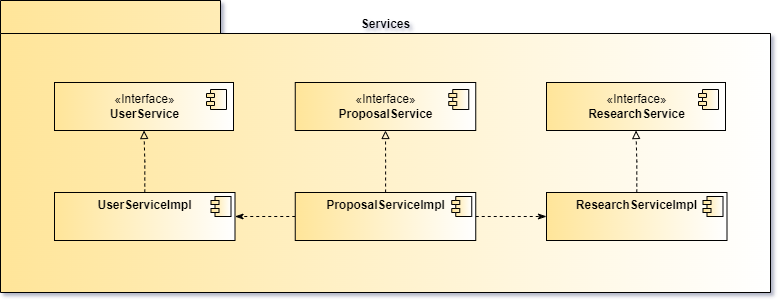
\includegraphics[scale=0.5]{Chapters/img/architecture/domain-services-example.png}
    \caption{Example of three existing services in CASCIFFO.}
    \label{fig:domain-services-example}
\end{figure}


Each service can communicate with their own associated repositories and other services, in addition to business logic, the request data validation and other exceptions are raised in this layer.

Most services have common similarities in terms of logic, replacing the repository used and data passed. Thus we will focus on three services: the proposal service, visit service and the user service. The first service is a pivotal point of the platform, interacting directly with one of the 'big' entities - the proposal entity, while the second one shows more common functionality to other services.


\subsubsection{User service}

The user service is to be mainly used by the user controller, the service itself utilizes other services as well as its dedicated repository - user repository.


The development of this service started with the design of the interface, from there, we ask the question of what operations are required from this type of service. Each client of the CASCIFFO platform requires a user account to be able to navigate through its features and use its capabilities. From this simple observation, the need for the registration and login operations arises. Doing a complete analysis of the features will find us with the following declaration of the user service interface as shown in the listing~\ref{lst:user-service-interface}

\begin{lstlisting}[
language={kt},
caption={User service interface.},
label={lst:user-service-interface}
]
interface UserService {
    //create operations
    suspend fun registerUser(userModel: UserModel) : BearerTokenWrapper
    //get operations
    suspend fun loginUser(userModel: UserModel): BearerTokenWrapper
    suspend fun getAllUsers() : Flow<UserModel?>
    suspend fun getUser(id: Int) : UserModel?
    suspend fun getAllUsersByRoleNames(roles: List<String>): Flow<UserModel>
    suspend fun searchUsers(name: String, roles: List<String>): Flow<UserModel?>
    suspend fun findUserByEmail(email: String): UserModel?
    //update operations
    suspend fun updateUser(user: UserModel): UserModel
    suspend fun updateUserRoles(roles: List<Int>, userId: Int): UserModel
    suspend fun notifyRoles(roles: List<Roles>, notificationModel: NotificationModel)
    //delete operations
    suspend fun deleteUser(userId: Int): UserModel
    suspend fun deleteUserRoles(roleIds: List<Int>, userId: Int): UserModel
}
\end{lstlisting}

This first iteration of the user service interface shows methods with the responsibility of registration, login, searching, updating, notifying and deleting user related data.
Another question that can be raised with this declaration is why do we have notification and user role manipulation here when their own services exist? This can be explained by seeing the implementation of the user service. The class implementing this interface that is used across the module is as named \lstinline{UserServiceImpl} and it's declaration can be viewed in the listing~\ref{lst:user-service-impl-declaration}

\begin{lstlisting}[
language={kt},
caption={User service implementation declaration.},
label={lst:user-service-impl-declaration}
]
@Service
class UserServiceImpl(
    @Autowired val userRepository: UserRepository,
    @Autowired val userRolesRepo: UserRolesRepo,
    @Autowired val userRolesAggregateRepo: UserRolesAggregateRepo,
    @Autowired val roleService: RoleService,
    @Autowired val notificationService: NotificationService,
    @Autowired private val encoder: PasswordEncoder,
    @Autowired val jwtSupport: JwtSupport
) : UserService { /*...*/ }
\end{lstlisting}

Through this short code, there are many details that require some attention, namely the new annotation \lstinline{@Service}. This annotation is a general-purpose stereotype where its semantics are left up to the developers and its context. It is also considered a specialization of \lstinline{@Component}, allowing the allowing for implementation classes to be auto detected through \textit{classpath} scanning. 

Moving to the class arguments it's observable that the service communicates with other parts of the module. Besides the service and repository arguments, the arguments \lstinline{enconder} and \lstinline{jwtSupport} are used for authentication purposes and will be further discussed in the authentication section~\ref{ch:impl:sec:be:subsec:authentication}.


The implementation of this class consists on overriding each method declared in the mentioned interface. 
The implementation of the method \lstinline{updateUserRoles} seen below in the listing~\ref{lst:user-service-impl-user-roles}.

\begin{lstlisting}[
language={kt},
caption={Add user roles method implementation.},
label={lst:user-service-impl-user-roles}
]
override suspend fun updateUserRoles(roles: List<Int>, userId: Int): UserModel {
    val user = getUser(userId) ?: throw ResponseStatusException(HttpStatus.BAD_REQUEST, "Utilizador com id [$userId] não existe!")
    if (roles.isEmpty()) return user
    val currentRoles = user.roles?.collectList()?.awaitFirstOrNull()
    val rolesToAdd = if (currentRoles.isNullOrEmpty()) roles
                    else roles.filter { r -> !currentRoles.any { cr -> r == cr.roleId!! } }
    if(rolesToAdd.isEmpty()) return user
    userRolesRepo
        .saveAll(rolesToAdd.map { //it: Int = roleId
            UserRoles(userId = userId, roleId = it) 
        })
        .subscribe()
    val updatedRoles = roleService
    .findByUserId(userId)
    .map { //it = UserRole(roleName, id)
    it.roleName!! 
    }.collectList()
    .awaitSingle()
    notificationService.createNotification(userId,
        NotificationModel(
            title = "Novos papéis adicionados.",
            description = "Papéis novos:\n\t " + updatedRoles.joinToString(", ") + ".",
            notificationType = NotificationType.USER_NEW_ROLES
        )
    )
    return getUser(userId)!!
}
\end{lstlisting}

This method is interesting because we can see the usage of other services in play as well as data validation and exception raising. The usage of \lstinline{ResponseStatusException} will be discussed further in section~\ref{ch:impl:sec:be:subsec:authentication}.

\subsubsection{Proposal service}

The proposal service is one of the most complex services in terms of business logic due to validation restrictions of the module. Just like every other service, the proposal service consists of two parts, the interface and implementation, the interface, shown in listing~\ref{lst:proposal-service-interface}, displays operations being exposed to consumers of this service.

\begin{lstlisting}[
language={kt},
caption={Proposal service interface.},
label={lst:proposal-service-interface}
]
interface ProposalService {
    //get operations
    suspend fun getProposalCount(): CountHolder
    suspend fun getAllProposals(type: ResearchType, pageRequest: PageRequest? = null): Flow<ProposalModel>
    suspend fun getProposalById(id: Int, loadDetails: Boolean = true): ProposalModel
    suspend fun getProposalStats(): Flow<ProposalStats>
    suspend fun getLatestModifiedProposals(n: Int): Flow<ProposalModel>
    //create operations
    suspend fun create(proposal: ProposalModel) : ProposalModel
    //update operations
    suspend fun updateProposal(proposal: ProposalModel) : ProposalModel
    suspend fun transitionState(proposalId: Int, nextStateId: Int, request: ServerHttpRequest): ProposalModel
    //delete operations
    suspend fun deleteProposal(proposalId: Int): ProposalModel
}
\end{lstlisting}

The complexity of this service lies mainly on the method \lstinline{transitionState} which is where the proposal transitions from its current state to a new one. To beging to analyze this method, we must first detail the constructor of the implementing class, displayed in listing~\ref{lst:proposal-service-impl-declaration}, as to know what we can work with. 

\begin{lstlisting}[
language={kt},
caption={Proposal service implementation declaration.},
label={lst:proposal-service-impl-declaration}
]
@Service
class ProposalServiceImpl(
    @Autowired val proposalAggregateMapper: Mapper<ProposalModel, ProposalAggregate>,
    @Autowired val proposalResearchRepository: ProposalResearchRepository
    @Autowired val proposalAggregateRepo: ProposalAggregateRepo,
    @Autowired val proposalRepository: ProposalRepository,
    @Autowired val proposalStats: ProposalStatsRepo,
    @Autowired val userService: UserService,
    @Autowired val stateService: StateService,
    @Autowired val researchService: ResearchService,
    @Autowired val partnershipService: PartnershipService,
    @Autowired val validationsService: ValidationsService,
    @Autowired val commentsService: ProposalCommentsService,
    @Autowired val notificationService: NotificationService,
    @Autowired val timelineEventService: TimelineEventService,
    @Autowired val stateTransitionService: StateTransitionService,
    @Autowired val investigationTeamService: InvestigationTeamService,
    @Autowired val proposalFinancialService: ProposalFinancialService,
    @Autowired val jwtSupport: JwtSupport,
) : ProposalService { /*...*/ }
\end{lstlisting}

From the declaration, we can observe the amount of services and repositories this service communicates with.
Focusing on the implementation of the method \lstinline{transitionState}, shown in the listing~\ref{lst:proposal-service-impl-transitionState}. 

\begin{lstlisting}[
language={kt},
caption={Signature and implementation of the transitionState method.},
label={lst:proposal-service-impl-transitionState}
]
@Transactional(rollbackFor = [ResponseStatusException::class])
override suspend fun transitionState(
    proposalId: Int,
    nextStateId: Int,
    request: ServerHttpRequest
): ProposalModel {
    val token = request.headers.getFirst(HttpHeaders.AUTHORIZATION)!!
    val bearer = BearerToken(token.substringAfter("Bearer "))
    val userEmail = jwtSupport.getUserEmail(bearer)
    val user = userService.findUserByEmail(userEmail)!!
    val userRoles = user.roles!!.map { it.roleName!! }.collectList().awaitSingle()
    val prop = getProposalById(proposalId, false)
    return handleStateTransition(prop, nextStateId, userRoles)
}    
\end{lstlisting}

In the signature of this method we can observe a new annotation \lstinline{@Transactional}. This annotation describes a transaction attribute on a method or class. 
It's present on this method and all others who's execution alters data in the database, through create, update or delete operations. The addition of the attribute \lstinline{rollbackFor} specifies the type of exception, in this case \lstinline{ResponseStatusException}, on which the entire transaction should trigger a rollback operation. By default the rollback is triggered via run time exceptions. A rollback operation is one of reverting the changes made within the context of a given transaction.

In the method \lstinline{transitionState}, up until the last line of \lstinline{return}, the user roles are fetched and passed to \lstinline{handleStateTransition()} where the validation occurs and actual transition is made. 
To dissect this method, we start with the validations, these can be observed in~\ref{lst:proposal-service-impl-transition-init}, the first validation call is made to the \lstinline{stateService} to verify whether \lstinline{nextStateId} corresponds to a possible and valid state. To briefly explain the method \lstinline{verifyNextStateValid}, it makes a database access to query the \lstinline{NextPossibleStates} table and verifies whether the aforementioned state id matches the column \lstinline{nextStateId} on any row.
The following validation, in case the proposal's type is a clinical trial and its current state is \lstinline{VALIDACAO_CF} which corresponds to the state validation of financial contract, in this context we must verify whether the financial contract is fully validated by both the financial and juridical department. 

Lastly we validate whether the next state corresponds to the final state in a proposal, in case it is, we perform a check on whether the financial component (includes both the protocol and financial contract validation) is fully validated. Assuming this is correct the research is automatically created followed with a notification to the investigation team.

In case any of these validations fail, an exception of type \lstinline{ResponseStatusException} is triggered which will then trigger the rollback mentioned previously. 

\begin{lstlisting}[
language={kt},
caption={Implementation of the handleStateTransition method 1 of 2.},
label={lst:proposal-service-impl-transition-init}
]
suspend fun handleStateTransition(
        proposal: ProposalModel,
        nextStateId: Int,
        role: List<String>
): ProposalModel {
    //initial variables
    val currState = stateService.findById(proposal.stateId!!)
    val nextState = stateService.findById(nextStateId)
    val isClinicalTrial = proposal.type === ResearchType.CLINICAL_TRIAL
    val stateType = if(isClinicalTrial) StateType.FINANCE_PROPOSAL
    else StateType.STUDY_PROPOSAL
    //validations
    nextState.roles = stateService.verifyNextStateValid(currState.id!!, nextStateId, stateType, role).toFlux()
    
    if(isClinicalTrial && currState.name == States.VALIDACAO_CF.name) {
            val check = validationsRepository.isPfcValidatedByProposalId(proposal.id!!).awaitSingle()
            if(!check) {
                throw ResponseStatusException(HttpStatus.BAD_REQUEST, "O contrato financeiro ainda não foi completamente validado!")
            }
        }
    if (stateService.isTerminalState(nextStateId, stateType)) {
        if (isClinicalTrial) {
            val fullyValidated = validationsRepository.isPfcFullyValidated(proposal.financialComponent!!.id!!).awaitSingle()
            if (!fullyValidated)
                throw ResponseStatusException(
                    HttpStatus.BAD_REQUEST,
                    "O contrato financeiro ainda não foi completamente validado!"
                )
        }
        createResearch(proposal, isClinicalTrial)
        notifyTeam(proposal.id!!,
            NotificationModel(
                title = if (isClinicalTrial) "Ensaio Clínico criado!" else "Estudo observacional criado!",
                description = "A proposta com a sigla ${proposal.sigla} foi validada!\n" +
                        "Como tal, o ${if (isClinicalTrial) "ensaio clínico" else "estudo observacional"} foi criado" +
                        " com sucesso, visita a página para preencheres os detalhes!",
                notificationType = NotificationType.RESEARCH_DETAILS,
                ids = convertToJson(listOf(Pair("researchId", proposal.researchId!!)))
            )
        )
    }
    //...
}
\end{lstlisting}

Upon successfully passing the validations, the time line events are checked in case there's any associated to a state that can now be validated followed by the creation of the transition and a notification of progress to the team members, as shown in listing~\ref{lst:proposal-service-impl-transition-impl}. To conclude, the proposal is updated with the new state, saved with the repository call \lstinline{proposalRepository.save(proposal)} and returned.


\begin{lstlisting}[
language={kt},
caption={Implementation of the handleStateTransition method 2 of 2.},
label={lst:proposal-service-impl-transition-impl}
]
suspend fun handleStateTransition(
    proposal: ProposalModel,
    nextStateId: Int,
    role: List<String>
): ProposalModel {
    //...
    if(proposal.timelineEvents != null) {
        updateTimelineEvent(proposal.timelineEvents!!, nextState.name!!)
    }
    stateTransitionService.newTransition(proposal.stateId!!, nextState.id!!, stateType, proposal.id!!)
    if(nextState.stateFlowType !== StateFlowType.TERMINAL) {
        notifyTeam(proposal.id!!,
            NotificationModel(
                title = "Progresso no estado de Proposta",
                description = "Proposta com sigla ${proposal.sigla!!} avançou para o estado ${nextState.name!!}",
                notificationType = NotificationType.RESEARCH_DETAILS,
                ids = convertToJson(listOf(Pair("proposalId", proposal.id!!))),
                viewed = false
            )
        )
    }
    proposal.stateId = nextState.id
    return proposalRepository.save(proposal).awaitSingle()
}
\end{lstlisting}


\subsection{Controllers}\label{ch:impl:sec:be:subsec:controllers}

The controller layer is where the HTTPS requests are handled, the routing of requests is handled by Spring's framework with the help of annotations that distinguish what controller handles which route and operation.
To build a controller class, the class needs to be annotated with \lstinline{@Controller} or in this case of a \textit{REST API} module, \lstinline{@RestController}. The main difference between the two annotations is that \lstinline{@RestController} indicates that the class is a controller where \lstinline{@RequestMapping} methods assume \lstinline{@ResponseBody} semantics by default.
The \lstinline{@RequestMapping} accepts a route path to serve as the base of the controller class, \lstinline{@ResponseBody} indicates the type of response, in this case, \lstinline{JSON} is used in all responses. 

When building the operations of a controller class, the methods that handle route requests, depending on the type of operation, need to be annotated with one of the following \lstinline{@Post}, \lstinline{@Put}, \lstinline{@Get}, \lstinline{@Patch} or \lstinline{@Delete}, each of these annotations take in an optional argument that represents the path of the route taking into account the base path if specified in \lstinline{@RequestMapping(path)} on the class. 

Each of the methods in a controller class can return an object or a \lstinline{ResponseEntity<Type>} for more flexibility in the structure of the response. In the reactive environment that\textit{Spring Webflux}~\cite{spring-webflux} provides, each return type should be inside a \lstinline{Mono} or \lstinline{Flux} stream.
The former represents a stream of one object, whereas the latter a stream of objects, from 0 to N objects. \lstinline{Mono} and \lstinline{Flux} represent streams of data using \textit{Reactor}, these data types can be chained together like building blocks in a declarative manner of programming. First the developer explicitly declares the behavior of the chain, with functions such as \lstinline{map(), filter(), groupBy(), flatMap()}. The execution of this chain only begins once the stream is subscribed to. 

Returning a \lstinline{Mono} or \lstinline{Flux} lets the Spring framework handle when its subscribed and structures the response data, whenever a conversion to \lstinline{JSON} happens the streams are automatically subscribed to.
While \lstinline{Mono} and \lstinline{Flux} are \textit{Spring Webflux}~\cite{spring-webflux}'s standard since it operates over \textit{Reactor}, \textit{Kotlin} also offers another way of dealing with streams, while implementing the back-end module \textit{Kotlin Coroutines} were preferred over \lstinline{Mono} and \lstinline{Flux} due to its \lstinline{async-await} nature and ease of use. To use \textit{Kotlin Coroutines} the functions need to have the \lstinline{suspend} keyword, i.e \lstinline{suspend fun functionName(params)}, in this way, instead of returning a \lstinline{Mono<Type>} we can return the \lstinline{Type} directly. When dealing with \lstinline{Flux} data types, \textit{Kotlin} offers an alternative called \lstinline{Flow<Type>}, the type \lstinline{Flow} has a similar set of operations and behavior to \lstinline{Flux}. To convert a stream of type \lstinline{Flux} to a \lstinline{Flow}, a simple call to the method \lstinline{asFlow()} applied to the \lstinline{Flux} stream will do the job.

A caveat of \lstinline{Flux} and \lstinline{Flow} occurs when returning objects with nested streams, (i.e returning a \lstinline{Flow} of object A that has a nested \lstinline{Flow} of object B in its instance), during \textit{Spring}'s automatic conversion from object to \lstinline{JSON}, the nested streams aren't represented properly, showing only a fetch status instead of the stream itself. In order to address this issue, a \acrfull{dto} representation of each entity model was created to hold lists instead of reactive streams. In conjunction with this, several mappers were created for the conversion of entity models to their respective DTO representations.


\subsubsection{Mono/Flux syntax vs Suspend function syntax}~\label{subsubsec:kotlin-coroutines}

To understand the concept of a suspend function we must first understand what are \textit{Kotlin coroutines}, since a suspend function is a coroutine itself.

A \textit{Kotlin coroutine}, taken to its literal name, co and routine, can be seen as a cooperative routine, meaning a conjunction of instructions (routine) that runs along (co) with other tasks. In other words, a coroutine is an instance of suspendable computation that can execute blocks of code in concurrency with other coroutines.
In this context of concurrent programming, we can find another and very common way of of dealing with concurrent tasks; threads. 

\textit{Kotlin coroutines} and threads are both ways of concurrent programming, but they have some significant differences.
A coroutine is conceptually similar to a thread, in the sense that it takes a block of code to run concurrently with the rest of the code. However, a coroutine is not bound to any particular thread. It may suspend its execution in one thread and resume in another one.~\cite{kotlin-coroutines-your-first}

According to the article by~\citename{kotlin-lightweight}{author}~\cite{kotlin-lightweight} one of the main differences between coroutines and threads is that coroutines are light-weight, while threads are heavy-weight. This means that coroutines use much less memory and computational resources than threads, and can therefore be more efficient when dealing with large numbers of concurrent tasks.

Another difference pointed out in the same article, is that coroutines are cooperatively scheduled, while threads are preemptively scheduled. This means that in a coroutine, the currently running coroutine must explicitly yield control to another coroutine, while in a thread, the scheduler can interrupt the currently running thread at any time and give control to another thread. We can say that unlike threads which are usually controlled by the operating system, coroutines are managed by the user in conjunction with the programming language. This makes coroutines easier to reason about and debug, since the control flow is more predictable.

Additionally, coroutines can be easily composed and used in a non-blocking manner, while threads require explicit synchronization mechanisms such as locks to avoid race conditions and deadlocks.

Now, with the concept of \textit{Kotlin coroutine} defined, we can move on to creating \textit{suspending functions}. 
To do this, we simply need to add the keyword \lstinline{suspend} before the declaration of the function, thus making it a \textit{suspending} function.

On the topic of syntax choice, \textit{Kotlin Coroutines} was favored due to the simplicity and clarity of the written code.
To illustrate the difference in syntax between the usage of \textit{Spring}'s \lstinline{Mono}/\lstinline{Flux} and \textit{Kotlin coroutines} we'll use a small portion of CASCIFFO's data model focusing on a proposal, its principal investigator and the states of a proposal. The entities in play will be \lstinline{Proposal}, \lstinline{User} - representing investigators - and \lstinline{Comment}. Following the context given, a proposal has one principal investigator and can have several comments made by other investigators. The data of a proposal is split in the database, when wanting to get the full details of a proposal, a query must also be made to fetch the \lstinline{User} and another to fetch the~\lstinline{Comment} associated to the proposal. Assuming a repository exists for each of these entities their names are their respective entities suffixed with \lstinline{Repo} we can write the following code to query the database and fetch the entities needed to build a proposal with nested entity of investigator and a list of comments.
Below is the representation of the method \lstinline{getProposalDetails} using \lstinline{Mono}/\lstinline{Flux} in listing~\ref{lst:mono-syntax} and using a \textit{Kotlin Coroutine} in listing~\ref{lst:suspend-syntax}.

\begin{lstlisting}[
    language=kt, 
    caption={Loading nested entities in an object using Mono/Flux syntax}, 
    label={lst:mono-syntax}
]
fun getProposalDetails(pId: Int): Mono<Proposal> {
    return personRepo
        //findById returns Mono<Proposal>
        .findById(pId) 
        // zipWith returns Mono<Tuple2<Proposal, User>>
        .zipWith(userRepo.findByProposalId(pId)) 
        .flatMap{ 
            it.t1.pInvestigator = it.t2.get()
            it.t1 //Proposal
        }
        // zipWith returns Mono<Tuple2<Proposal, (Mutable)List<Comment>>
        .zipWith(commentsRepo.findAllByProposalId(pId).collectList()) 
        .flatMap {
            it.t1.comments = it.t2.get().map{e ->  commentsMapper.mapToDto(e) }
            it.t1
        }
}    
\end{lstlisting}


\begin{lstlisting}[
    language=kt, 
    caption={Loading nested entities in an object using suspend function syntax},
    label={lst:suspend-syntax}]
suspend fun getProposalDetails(pId: Int): Person {
    val proposal = proposalRepo.findById(pId).awaitSingle()
    person.pInvestigator = userRepo.findByProposalId(pId).awaitSingle()
    //here comments was changed from type Flux<Comment> to Flow<Comment>
    person.comments = commentsRepo.findAllByPersonId(pId).asFlow()
    return proposal
}    
\end{lstlisting}


\subsection{Mappers}\label{ch:impl:sec:be:subsec:mappers}

Mappers are crucial tool in any application, allowing the conversion of one data type into another and hiding the complexity of such operation. 

A single generic interface was created with two simple methods which can be observed in listing~\ref{lst:mother-mapper}, from which all other mappers implement.

\begin{lstlisting}[
language={kt},
caption={Mapper interface.},
label={lst:mother-mapper}
]
interface Mapper<Model, DTO> {
    suspend fun mapDTOtoModel(dto: DTO?): Model
    suspend fun mapModelToDTO(model: Model?): DTO
}
\end{lstlisting}

An implementation of this interface and be seen in the mapper below in listing~\ref{lst:example-mapper}. By comparing both the interface and implementation of the mapper we can observe that only the implementation has the annotation \lstinline{@Component}. This annotation tells \textit{Spring} which classes can be scanned and used for dependency injection, this topic will be approached in more detail in the subsection~\ref{ch:impl:sec:be:subsec:authentication}.

\begin{lstlisting}[
language={kt},
caption={Mapper for state entity.},
label={lst:example-mapper}
]
@Component
class StateMapper: Mapper<State, StateDTO> {
    override suspend fun mapDTOtoModel(dto: StateDTO?): State {
        throw NotImplementedError("Left blank on purpose.")
    }

    override suspend fun mapModelToDTO(model: State?): StateDTO {
        if(model == null) return StateDTO()
        return StateDTO(
            id = model.id,
            name = model.name,
            nextInChain = model.nextStates?.collectList()?.awaitSingleOrNull(),
            roles = model.roles!!.collectList().awaitSingleOrNull(),
            stateFlowType = model.stateFlowType!!
        )
    }
}    
\end{lstlisting}

Using Spring's powerful dependency injection, the services and controllers which use mappers don't need to know their specific name, we only need to set the correct types for \lstinline{Model} and \lstinline{DTO}. For example if we want to use the state mapper implementation~\ref{lst:example-mapper}, we pass it as a constructor argument to a class as such \lstinline{@Autowired val stateMapper: Mapper<State, StateDTO>}. The \lstinline{@Autowired} annotation indicates that a property should be injected via Spring's dependency injection mechanic.

During the mapping phase, nested objects of type \lstinline{Flux} or \lstinline{Flow} are subscribed to and subsequently transformed into lists that can be represented in \textit{JSON}.

Each mapping conversion from DTO to Model and vice versa are called within the controllers.


\subsection{Authentication}\label{ch:impl:sec:be:subsec:authentication}

On top of these layers lies Spring's own framework, and in it the Web Filters. Web Filters are methods that run during an incoming request. Through Spring's framework, they intercept and perform operations with the request data before control is given to a controller handler. 
These Web Filters are especially useful to perform authentication operations on the incoming requests.


The authentication was implemented with \acrfull{jwt}, each request that requires authentication must have a valid \acrshort{jwt} in the header 'Authentication' of the request. This \acrshort{jwt} in addition to the standard fields, also holds user information, namely the user email that is used to uniquely identify each user. 
To further security, a role-based access control was defined as mentioned previously in the document. This can be implemented in a few steps, first and foremost is to implement\textit{Spring Webflux}~\cite{spring-webflux}'s \lstinline{ReactiveUserDetailsService}, which is responsible for fetching a user based on a passed argument \lstinline{username}, this method will be called during the interception of a request that requires authentication. The next step is to create an authentication manager that implements \lstinline{ReactiveAuthenticationManager} and overriding the method \lstinline{authenticate}, this manager is responsible for extracting and validating the information from a \acrshort{jwt}. Note that both the classes that implement these interfaces need to be annotated with \lstinline{@Component}. The need for the annotations comes from a useful feature of \textit{Spring}'s framework, dependency injection, by annotating these classes with \lstinline{@Component} or methods with \lstinline{@Bean} allows \textit{Spring} to scan and detect the classes and auto inject them into other parts of the code where they are passed as arguments for methods or constructors. This classes then become \textit{candidates} for injection depending on the context. 

\textit{Spring} taking control of this aspect of the code, can be referred as \acrfull{ioc} where a framework takes control of a portion of the program or code, instead of the programmer explicitly controlling it.

 
To make use of this newly created components we need to add the authentication manager to the \lstinline{WebFilter} chain that can be accessed and configurable from a class annotated with \lstinline{@Configuration} and implementing the method \lstinline{springSecurityFilterChain}, annotated with \lstinline{@Bean}. 
This method receives an argument \lstinline{http} of type \lstinline{ServerHttpSecurity} and should also receive the created authentication manager component as an argument. 
Finally to add it to the \lstinline{WebFilter} chain, the method \lstinline{addFilterAt()} is used, applied to the argument \lstinline{http}. 

This describes how a \acrshort{jwt}'s information is extracted and validated, to implement a role-based access control, one can choose Spring's annotation-based authentication, by annotating the required methods or controller classes with \lstinline{@PreAuthorize(string)}. The passed argument is a function name alongside its arguments, in this context, the most adequate ones would be \lstinline{hasAuthority()} or \lstinline{hasAnyAuthority()}. Another possible way of implementing this requirement is by utilizing the \lstinline{http} argument mentioned previously inside the method \lstinline{springSecurityFilterChain} and programmatically add these rules to each route, as shown in the coding listing~\ref{lst:spring-security}. By utilizing the methods \lstinline{authorizeExchange()} followed by \lstinline{pathMatchers(route)} and applying \lstinline{hasAnyAuthority(authorities)} or \lstinline{hasAuthority(authority)}. An authority is simply a constant with a string value specifying a role, for context, some of the authorities used were \lstinline{SUPERUSER_AUTHORITY} and \lstinline{UIC_AUTHORITY}. 


\begin{lstlisting}[
    language={kt}, 
    caption={Configuration of spring security filter chain},
    label={lst:spring-security}]
@Bean
fun springSecurityFilterChain(
    converter: JwtServerAuthenticationConverter,
    http: ServerHttpSecurity,
    authManager: JwtAuthenticationManager
): SecurityWebFilterChain {

    val jwtFilter = AuthenticationWebFilter(authManager)
    jwtFilter.setServerAuthenticationConverter(converter)

    http
        .addFilterAt(jwtFilter, SecurityWebFiltersOrder.AUTHENTICATION)

    //example of routing configuration
    http
        .authorizeExchange()
        .pathMatchers(HttpMethod.GET, ENDPOINTS_URL)
            .permitAll()
        .pathMatchers(HttpMethod.POST, ENDPOINTS_URL)
            .hasAnyAuthority(SUPERUSER_AUTHORITY, UIC_AUTHORITY)
        .pathMatchers(HttpMethod.DELETE, ENDPOINTS_URL)
            .hasAuthority(SUPERUSER_AUTHORITY)
             
    //other http configurations
    ...
            
    return http.build()
}
\end{lstlisting}

Both the discussed approaches were experimented with, having settled with programmatically adding new rules to each route as needed. This choice was made based on performance issues with the annotation-based authentication, the annotation \\\lstinline{@PreAuthorize()} was adding an overhead of up to 1 second per request, whereas programmatically this issue was not observed. The cause could inherently be due to~\textit{Spring Webflux}~\cite{spring-webflux}, since the annotation \lstinline{@PreAuthorize} is more commonly used with \textit{Spring Web}.


\subsection{Exception handling}~\label{ch:impl:sec:be:subsec:exceptions}

On the topic of business rules, in case one is broken, an exception must be raised with information regarding the cause. Business rules are defined in the service layer and conversely it is where incoming requests are validated before performing the requested operation. If the information passed along the request isn't valid, an exception is manually thrown with an appropriate \lstinline{HTTP status} and a reason, since the back-end module exposes a REST API. 


With exceptions being raised whenever there's invalid data on incoming requests, the response must come with appropriate information on why the request failed or was rejected. For example, when requesting a resource that requires authentication yet the request sent none, the response will provide sufficient information so the one that made the request knows that for accessing that specific resource, it is also required to send authentication and how to send it.


To handle these exceptions and others that can occur during run-time, for example a database integrity violation or in case the database is unreachable among other possible run-time exceptions we can make use of great features provided by \textit{Spring}'s framework. We first looked at utilizing custom exceptions annotated with \lstinline{@ResponseStatus}, by annotating a class that extends \lstinline[keywordstyle=\color{black},commentstyle=\color{black},stringstyle=\color{black}]{Exception}, we can define the response status code and the reason that caused the exception to be thrown, as illustrated by the listing~\ref{lst:ex-rsp-status}. 

\begin{lstlisting}[
    language={kt},
    label={lst:ex-rsp-status},
    caption={Example of an exception annotated with @ResponseStatus}
]
@ResponseStatus(
    code = HttpStatus.NOT_FOUND, 
    reason = "Specified resource Id doesn't exist."
)
class ResourceNotFoundException(): Exception()
\end{lstlisting}

This approach is simple and makes use of \textit{Spring}'s automatic converter to \textit{JSON}. The issue lies in its simplicity, it doesn't allow us to change anything other than reason and status code, the body itself is handled by \textit{Spring}, an example of an answer can be observed in the code listing~\ref{lst:ex-response-example}. 
We would also need to create several exception classes for each edge case that requires an exception to be thrown.

\begin{lstlisting}[
    language={json},
    label={lst:ex-response-example},
    caption={Example response using \textit{Spring}'s automatic response converter.}
]
"{
    "timestamp": "2022-11-09T12:24:21.609+00:00",
    "path": "/proposals/999",
    "status": 404,
    "error": "Not Found",
    "message": "Specified resource Id doesn't exist.",
    "requestId": "c0d35eab-2"
}"
\end{lstlisting}


One other possible solution was to create specific exception handlers, using the annotation \lstinline{@ExceptionHandler(SampleException::class)} on a method and passing the class type of exception to catch as its argument, we can process specific exceptions locally within the controller classes themselves, as shown in listing~\ref{lst:sample-controller-handler}. This resolves issue of the first approach in the sense that we can make use of the incoming request and outgoing response to write our own defined response body. 
The trade offs, however, come at a cost of maintenance, the exception handlers will be tightly coupled to their controllers and one exception handler can only process one type of exception for that particular controller.

\begin{lstlisting}[
language={kt},
caption={Sample controller with exception handler},
label={lst:sample-controller-handler}
]
class FooController{
    //...
    @ExceptionHandler({ CustomException1.class, CustomException2.class })
    fun handleException() {
        //logic
    }
}    
\end{lstlisting}

Another analyzed approach was the implementation of \lstinline{ErrorWebExceptionHandler} and overriding the method \lstinline{override fun handle(ServerWebExchange, Throwable): Mono<Void>}. The purpose of this method is to catch any exceptions not handled by the exception handlers mentioned earlier. In the context of this method we have access to the argument of type \lstinline{ServerWebExchange} which includes in its properties the request, the response and other useful information about the this particular connection that resulted in an exception. Here we are also able to access and customize the body property of the response as we wish.

Yet another studied approach was the usage of classes annotated with \\\lstinline{@RestControllerAdvice}, these classes can intercept exceptions when controllers, respectively annotated with \lstinline{@RestController} raise exceptions. With this class we can centralize all exception handlers in one place, decoupling the controllers of their exception handlers and moving the latter here. 

The last studied solution was the usage of the exception class  \lstinline{ResponseStatusException}, which on the contrary to the first mentioned approach, the exceptions are defined and thrown locally within their scope. This reduces the amount of exception classes since one type of exception can be used for any issue. The trade off of this approach is be the increased difficulty of code management and duplicated code inside the code blocks that raise exceptions. 

The final solution consisted in a mix and match of the described approaches. 
A global exception handler was created by utilizing the creation of a class annotated with \\\lstinline{@RestControllerAdvice}. For specific exceptions, the usage of a method annotated with \lstinline{@ExceptionHandler} and accepting the argument \lstinline{ResponseStatusException::class} facilitated in manipulating the response body. With this solution, we benefit from global exception handling and decoupled controllers. This solution can be observed in listing~\ref{lst:global-exception-handler}.

\begin{lstlisting}[
language={kt},
caption={Implementation of a global exception handler.},
label={lst:global-exception-handler}
]
@RestControllerAdvice
class GlobalExceptionController {

    val logger = KotlinLogging.logger {  }

    @ExceptionHandler(ResponseStatusException::class)
    suspend fun handleResponseStatus(ex: ResponseStatusException, req: ServerHttpRequest, rsp: ServerHttpResponse): GenericExceptionDTO {
        val exDTO = GenericExceptionDTO(
            path = req.path.toString(),
            uri = req.uri.toString(),
            reason = ex.reason ?: "Internal Error",
            status = ex.rawStatusCode
        )
        logger.error {exDTO}
        rsp.statusCode = ex.status
        rsp.headers.contentType = MediaType.APPLICATION_JSON
        return exDTO
    }
}
\end{lstlisting}



\section{Front-end module}~\label{ch:impl:sec:fe}

In this section, an examination of the \acrlong{fe} module development is made. Starting with the reasons for choosing each tool in this process, then the inner workings of each layer in this module, and concluding with how functional requirements are met.


It is structured as follows:

\begin{itemize}
    \item Framework Stack~\ref{ch:impl:sec:fe:subsec:framework-stack} - describes the frameworks used for the development of the \acrlong{fe} module;
    \item Configuration \& Required Modules~\ref{ch:impl:sec:fe:subsec:config-and-modules} - Describes the configuration and used modules to build the \acrlong{fe} module;
    \item Model Layer~\ref{ch:impl:sec:fe:subsec:model-layer} - Describes the model layer;
    \item Services Layer~\ref{ch:impl:sec:fe:subsec:service-layer} - Describes the service layer;
    \item View Layer~\ref{ch:impl:sec:fe:subsec:view-layer} - Describes the view layer;
    \item Security~\ref{ch:impl:sec:fe:subsec:auth} - describes the steps taken to implement authentication and role based permission in the \acrlong{fe} module;
\end{itemize}


\subsection{Framework Stack}~\label{ch:impl:sec:fe:subsec:framework-stack}

The \acrshort{fe} module was developed using \textit{ReactJs}, version 18, mainly due to its popularity and ease of use alongside a super set of \textit{JavaScript}; \textit{TypeScript}, version 4. The module is built using a node package manager, the popular \textit{npm}. 

During development the tool \textit{npx webpack} was used to deploy the module, benefiting from its \textit{Watch} feature where whenever a change is made on a source file the code is compiled without needing to manually compile and deploy. 


Using the tool \textit{npx} and \textit{create-react-app} we obtain a template project with some required settings for this module, namely, having the project in \textit{TypeScript} and having it adapted to be a \acrshort{pwa}. This is achieved through the command \lstinline[keywordstyle=\color{black},commentstyle=\color{black},stringstyle=\color{black}]{npx create-react-app front-end --template cra-template-pwa-typescript}, which creates a ready to go application in the folder \lstinline[keywordstyle=\color{black},commentstyle=\color{black},stringstyle=\color{black}]{front-end} using \textit{TypeScript} and \textit{ReactJs} with the requirements to be a \acrshort{pwa}.

This module was developed to be a \acrfull{spa} and consists of three main components, the View, Model and Service.

\subsection{Configuration \& Required Modules}~\label{ch:impl:sec:fe:subsec:config-and-modules}

With the ready to application from the mentioned command, we are met with two important files for configuration and setting required modules - \lstinline{tsconfig.js}(viewed in listing~\ref{lst:ts-config}) and \lstinline{package.json}(a brief showcase can viewed in listing~\ref{lst:ts-package-json} with the entire file available in the GitHub repository). The former refers to the typescript compiler options while the latter includes the required modules for development and production.

\begin{lstlisting}[
language={json},
caption={TypeScript compileer configuration file.},
label={lst:ts-config}
]
{
  "compilerOptions": {
    "target": "es6",
    "lib": [
      "dom",
      "dom.iterable",
      "esnext"
    ],
    "allowJs": true,
    "skipLibCheck": true,
    "esModuleInterop": true,
    "allowSyntheticDefaultImports": true,
    "strict": true,
    "forceConsistentCasingInFileNames": true,
    "noFallthroughCasesInSwitch": true,
    "module": "esnext",
    "moduleResolution": "node",
    "resolveJsonModule": true,
    "isolatedModules": true,
    "noEmit": true,
    "jsx": "react-jsx"
  },
  "include": [
    "src"
  ]
}
\end{lstlisting}


Out of the properties present in the \lstinline{tsconfig.json} file~\ref{lst:ts-config}, some of the most impactful are the following:
\begin{itemize}
    \item \lstinline[keywordstyle=\color{black},commentstyle=\color{black},stringstyle=\color{black}]{"target": "es6"} - This option specifies the target compatibility of the \textit{JavaScript} generated by the \textit{TypeScript};

    \item \lstinline[keywordstyle=\color{black},commentstyle=\color{black},stringstyle=\color{black}]{"include": ["src"]} - This option specifies that the \textit{TypeScript} compiler should only include files inside the \lstinline{src} folder and its sub-folders. It takes in an array of strings, each denoting what folder should be included in the compilation.
\end{itemize}


The \lstinline{package.json} file, displayed in listing~\ref{lst:ts-package-json}, is a plain \textit{JSON} file and it contains information about the project, its dependencies, scripts, and version. The \lstinline[keywordstyle=\color{black},commentstyle=\color{black},stringstyle=\color{black}]{"dependencies"} property lists the packages that the project depends on in order to function properly. 
These are packages that are required to run the project in production. Each dependency is represented by the package's name and version number. The version number can be specified in a variety of ways, such as an exact version number (e.g. "1.2.3"), a range of versions (e.g. "\^~1.2.3" or "~1.2.3"), or the keyword "latest" to always use the latest version of the package. To make sure the project stays consistent we used the pattern "\^~1.2.3" so the dependency can be updated according to its major version, the use of a caret "\^" version prefix indicates that any minor version that is compatible with the specified major version can be used.


The \lstinline[
    keywordstyle=\color{black},
    commentstyle=\color{black},
    stringstyle=\color{black},
]{"devDependencies"} property lists the packages that are required for development only, such as testing and building libraries, which in this case contains the \lstinline{react-scripts} used for building and compiling the application. Once compiled this dependency is no longer required, thus having it included in this property makes it so the production build isn't bloated with this package.

When the command \lstinline{run npm install} is executed from the project directory, it will install all the packages listed in both mentioned property fields and create a \lstinline[
        keywordstyle=\color{black},
        commentstyle=\color{black},
        stringstyle=\color{black},
    ]{node_modules} folder that contains all the installed packages, along with their own dependencies.

During development the mentioned command was used with no other options, however, to deploy using a production build, we can pass the flag \lstinline[
        keywordstyle=\color{black},
        commentstyle=\color{black},
        stringstyle=\color{black},
    ]{--only=production} which will tell Node to skip the dependencies listed in the property \lstinline{devDependencies}.

Along with these two properties, have another two that restrict the environment the project can run on. These are:
\begin{itemize}
    \item \lstinline[keywordstyle=\color{black},commentstyle=\color{black},stringstyle=\color{black}]{"engines"} - Indicates the version of \textit{NodeJs} and \textit{npm} that the project requires to run properly.
    \item \lstinline[keywordstyle=\color{black},commentstyle=\color{black},stringstyle=\color{black}]{"enginesStrict"} - Specifies whether the package should error if the version of \textit{NodeJs} or \textit{npm} is not compatible with the version specified in the \lstinline[keywordstyle=\color{black},commentstyle=\color{black},stringstyle=\color{black}]{"engines"} field. 
\end{itemize}

\begin{lstlisting}[
language={json},
caption={Package.json configuration file.},
label={lst:ts-package-json}
]
{
  "name": "casciffo-front-end",
  "version": "1.0.0",
  "private": true,
  "dependencies": {
    "axios": "^1.2.1",
    "bootstrap": "^5.2.3",
    "chart.js": "^4.1.1",
    "file-saver": "^2.0.5",
    "react": "^18.2.0",
    "react-bootstrap": "^2.7.0",
    "react-chartjs-2": "^5.1.0",
    "react-chrono": "^1.20.0",
    "react-csv": "^2.2.2",
    "react-data-table-component": "^7.5.3",
    "react-dom": "^18.2.0",
    "react-router-bootstrap": "^0.26.2",
    "react-router-dom": "^6.6.0",
    "react-toastify": "^9.1.1",
    "serve": "^14.1.2",
    "typescript": "^4.9.4",
    //other dependencies
  },
  "devDependencies": {
    "react-scripts": "^5.0.1"
  },
  "scripts": {
    "start": "react-scripts start",
    "build": "react-scripts build",
    "test": "react-scripts test",
    "eject": "react-scripts eject"
  }
  "engines": {
    "node": "18.x",
    "npm": "8.x"
  },
  "engineStrict": true,
  //other configurations
}
\end{lstlisting}


In addition to these we also need a way to specify whether the current build is for development or production, to indicate which base URL the \acrshort{fe} should use. This is especially relevant during development when both the project's modules aren't bundled together and instead running as two separate applications, such as in two different \textit{Heroku} containers.
This can be done by creating two files, \lstinline{.env.development} and \lstinline{.env.production}, where we set the needed variables during on the type of build. Since we created the project using the command \lstinline[keywordstyle=\color{black},commentstyle=\color{black},stringstyle=\color{black}]{npm create-react-app}, the project uses an environment variable \lstinline{NODE_ENV}, will look for these two environments depending on the type of command being used to start the build. The variable \lstinline{NODE_ENV} cannot be changed manually, however, the command \lstinline{npm start} makes it so the variable \lstinline{NOVE_ENV} will always have the value of "development" and therefore look for \lstinline{.env.development} while the command \lstinline{npm run build} will have \lstinline{NODE_ENV} with the value of "production" and thus make it scan for \lstinline{.env.production}.  In case we need to other variables, we can set them prior to running the command, granted that the variable must be prefixed with \lstinline{REACT_APP_}.


\subsection{Model Layer}~\label{ch:impl:sec:fe:subsec:model-layer}

The model layer is where all model entities are held. 
The entities are represented through interfaces, since we only need to specify the shape of the object being worked on and don't expect any type of internal behavior. An example of these interfaces can be seen in listing~\ref{lst:fe-model-impl-example}.
Interfaces were chosen over classes since we don't need any behavior attached to a model entity. In contrast, type alias and interfaces are very similar in \textit{TypeScript} with the key distinction being that a type cannot be redefined to add new properties versus an interface which can be redefined to extend new properties or methods.

\begin{lstlisting}[
language={ts},
caption={User Model Interface.},
label={lst:fe-model-impl-example}
]
export interface UserModel {
    userId ?: string,
    name?: string,
    email?: string,
    password?: string,
    roles?: UserRoleModel[],
}
\end{lstlisting}

These model interfaces are used by the service and view layer.


\subsection{Service Layer}~\label{ch:impl:sec:fe:subsec:service-layer}
The service layer is where data is requested via HTTP to the \acrshort{be} module.

All services are stateless and responsible for requesting data related to certain entities. Services may also communicate with each other to form an aggregate service, for the ease and convenience of centralizing the dependencies of a view component into one single aggregate.

Requests made over HTTP use the browser built-in \lstinline{fetch} function. This function takes in one mandatory argument, the URL, and optional arguments specifying the options to be considered, such as whether the request being made is a POST or GET, as well as defining the headers and body of said request.

Each service makes use of this function indirectly through a made utility class containing several utility methods. In the listing~\ref{lst:fe-util-fetch} we can observe the utility methods used to fetch data. 


\begin{lstlisting}[
language={ts},
caption={Utility fetch methods.},
label={lst:fe-util-fetch}
]
const APPLICATION_CONTENT_TYPE = 'application/json'
const HEADER_ACCEPT_JSON: [string,string] = ['Accept', APPLICATION_CONTENT_TYPE]
const HEADER_CONTENT_TYPE: [string,string] = ['Content-Type', APPLICATION_CONTENT_TYPE]
const HEADER_AUTHORIZATION = (token: string): [string,string] => ['Authorization', 'Bearer ' + token]
const HTTP_STATUS_NO_CONTENT = 204

export function httpGet<T>(url: string) : Promise<T> {
    return _httpFetch(url, 'GET')
}
export function httpDelete<T>(url: string, body: unknown = null) : Promise<T> {
    return _httpFetch(url, 'DELETE', [HEADER_CONTENT_TYPE], body)
}
export function httpPost<T>(url: string, body: unknown): Promise<T> {
    return _httpFetch(url, 'POST', [HEADER_CONTENT_TYPE], body)
}
export function httpPostNoBody<T>(url: string): Promise<T> {
    return _httpFetch(url, 'POST')
}
export function httpPut<T>(url: string, body: unknown = null): Promise<T> {
    return _httpFetch(url, 'PUT', [HEADER_CONTENT_TYPE], body)
}
\end{lstlisting}


As observed in the listing, each of these methods use the function \lstinline{_httpFetch}, as viewed in listing~\ref{lst:fe-util-fetch-main}, this is where the built-in \lstinline{fetch} function is wrapped. This function first prepares adds to the headers array the content type of the request, the type being \lstinline{application/json} as observed in the previous listing(\ref{lst:fe-util-fetch}). The communication between the \acrshort{fe} and \acrshort{be} over HTTP consist in requests where data is passed in \textit{JSON} format.

Afterwards, the local storage is accessed to retrieve a \lstinline{token}, this token is the token sent back by the \acrshort{be} module upon a successful login, upon which it is stored in the browser's local storage.
The token is required to be present in the header \lstinline{Authorization}, prefixed by \lstinline{Bearer} since it is a bearer token, to able to perform a number of operations within the platform, especially those that involve database write operations. Following the flow of control of the method, the options, named \lstinline{opt}, is created with the previously set headers and the argument \lstinline{url}, in case the \lstinline{body} is not null, it is included in the options of the request, and finally the call to the \acrshort{be} is made through the function \lstinline{fetch}. We can explicitly note that this function (\lstinline{fetch}) is asynchronous as it returns a \lstinline{Promise} of data. As a final note upon receiving a response from the \acrshort{be}, the response is then checked for errors, in which case we retrieve the content of the message through \lstinline{rsp.text()} and not \lstinline{rsp.json()}. The former method reads the body as if it were a string thus being better suited to handle any type of possible error where the response body is not certain while the latter method expects the body to be formatted in \textit{JSON}.


\begin{lstlisting}[
language={ts},
caption={Utility fetch wrapper method implementation.},
label={lst:fe-util-fetch-main}
]
async function checkAndRaiseError(rsp: Response): Promise<Response> {
    if(!rsp.ok) {
        const status = rsp.status
        const body = await rsp.text()
        throw new MyError(
            JSON.parse(body).reason, status)
    }
    return rsp
}

function _httpFetch<T>(
    url: string,
    method: string,
    headers: [string, string][] = [],
    body: unknown = null
): Promise<T> {
    headers.push(HEADER_ACCEPT_JSON)
    const token = localStorage.getItem(TOKEN_KEY)
    if(token != null) {
        const userToken = JSON.parse(token) as UserToken
        headers.push(HEADER_AUTHORIZATION(userToken?.token))
    }
    const opt : RequestInit = {
        headers: headers,
        method: method
    }
    if(body != null) {
        opt.body = JSON.stringify(body)
    }
    return fetch(url, opt)
        .then(checkAndRaiseError)
        .then(rsp => rsp.status === HTTP_STATUS_NO_CONTENT ? rsp : rsp.json())
}
\end{lstlisting}


With the utility methods explained, the services can be easily described with the short piece of code observable in listing~\ref{lst:fe-service-impl}. All the methods in each service behaves in a similar way to it, prepare the request URL and call the utility function.

\begin{lstlisting}[
language={ts},
caption={User Service implementation snippet.},
label={lst:fe-service-impl}
]
export class UserService {
    fetchAll() : Promise<Array<UserModel>> {
        return httpGet(ApiUrls.usersUrl)
    }
    fetchUser(userId: string): Promise<UserModel> {
        const url = ApiUrls.userDetailsUrl(userId)
        return httpGet(url)
    }
    login(userModel: userModel) : Promise<UserToken> {
        return httpPost(ApiUrls.userLoginUrl, userModel)
    }
    register(userModel: UserModel): Promise<UserToken> {
        return httpPost(ApiUrls.userRegisterUrl, userModel)
    }
    addRolesToUser(userId: string, roleIds: number[]): Promise<UserModel> {
        const url = ApiUrls.userRolesUrl(userId)
        return httpPut(url, roleIds)
    }
    removeUserRoles(userId: string, roleIds: number[]): Promise<UserModel> {
        const url = ApiUrls.userRolesUrl(userId)
        return httpDelete(url, roleIds)
    }  
    //other request methods ...
}
\end{lstlisting}


\subsection{View Layer}~\label{ch:impl:sec:fe:subsec:view-layer}

The view layer is where the user interaction begins, with the framework \textit{ReactJs}~\cite{reactjs}, the \acrshort{ui} is built with Components. A component can be understood as a building block of a page, it is reusable and provides ways to handle state and logic in an isolated manner. Conceptually, components are like JavaScript functions. They accept arbitrary inputs, \lstinline{props}, and return React elements describing what should appear on the screen. 
Furthermore, a component can also be divided into two categories: state-full and stateless components, depending on whether they manage state or not. The usage of state in components with state can be represented with the react hook \lstinline{useState<Type>(initialValue)}, whereas a stateless component, commonly referred to as functional component, does not handle state and only encapsulates logic and/or returns a React element based on the arguments it receives within the \lstinline{props} property. Functional components are useful for re-usability and code readability.

Each component is created in the virtual DOM, a concept that represents the \acrshort{ui} in memory as a lightweight, abstract tree of nodes. When the state of a React component changes, React updates the virtual DOM instead of the actual DOM. Then, React calculates the difference between the previous virtual DOM and the new virtual DOM, and applies the smallest possible updates to the actual DOM. This behavior allows pages to only re-render components that have been updated instead of the whole page, thus reducing the load on the browser and leading to an increased performance in page response time.

Each component goes through a lifecycle of events, beginning when the component is created, followed when it's data is updated and finally when it's destroyed. These events in a class component correspond, respectively, to the functions:
\begin{itemize}
    \item \lstinline{componentDidMount()} - Called when the component is mounted and its initial render has completed;
    \item \lstinline{componentDidUpdate()} - Called whenever there is a change in the data of the component which causes a re-render;
    \item \lstinline{componentWillUnmount()} - Called before the component is unmounted, meaning removed from the DOM.
\end{itemize}

In the context of the \acrshort{fe} module, function based components were used and in such components, instead of these methods, \textit{React hooks} are used instead. The most notable \textit{React hooks} are: \lstinline{useState()} - used to declare "state variables", a call to this method returns the state variable and a function to set a new value to the variable that will trigger a re-render of the component; \lstinline{useEffect()} - used to perform logic after the component has rendered, this method takes in a callback as first argument that will be executed upon a successful render of the component and can be customized to trigger only on certain state variable changes. This is achieved by passing a dependencies array as a second argument, where each array value corresponds directly to the variable to observe, in the case the dependencies array is empty or depends only on props, the provided callback will only execute on the initial render of the component.

In conjunction with React, other JavaScript libraries that offer a base of components and styles were used to build the \acrshort{ui}, namely \textit{React Bootstrap} for components and \textit{Mazer UI}~\footnote{\url{https://github.com/zuramai/mazer}}~\label{fn:mazer-ui} for styling.

With how each \acrshort{ui} page is created explained, we need to address how we can navigate between pages, which leads us to \textit{React Router}. \textit{React Router} is a library that provides the capability of mapping URLs to specific components, making it easier to keep track of and manage the application as it grows. Additionally, \textit{React Router} also supports dynamic routing, allowing the creation of routes with variables, such as \lstinline[keywordstyle=\color{black},commentstyle=\color{black},stringstyle=\color{black}]{/proposal/:pId} where \lstinline{:pId} identifies a variable named \lstinline{pId}, this variable can then be accessed by using the \textit{React} function \lstinline{useParams()}. This function returns an object with all variables mapped as properties, as such, to access the previous \lstinline{pId} we need only to retrieve the property \lstinline{pId} from the object returned by the function in question.

To create a route using JSX syntax, we can utilize the following snippet \lstinline[keywordstyle=\color{black},commentstyle=\color{black},stringstyle=\color{black}]!<Route path={"/"} element={Component}/>!, where the property \lstinline{path} indicates the URL and the \lstinline{element} property the component that should be displayed once the designated URL is in place.
This feature is heavily used in the routing management of the \acrshort{fe} module, as observed in listing~\ref{lst:react-routing} where a snippet of the creation of routes is shown. 

\begin{lstlisting}[
language={ts},
caption={Routes snippet for FE module.},
label={lst:react-routing}
]
export function CreateRoutes() {

return (
    <Routes>
        <Route path={"/"} element={RequiresAuth(<Dashboard statisticsService={new StatisticsService()}/>)}/>
        <Route path={"/login"} element={<Login UserService={new UserService()}/>}/>
        <Route path={"/logout"} element={<Logout/>}/>
        <Route path={"/propostas/:proposalId"}
               element={RequiresAuth(<ProposalDetailsPage proposalService={new ProposalAggregateService()}/>)}
        />
        <Route path={"/ensaios/:researchId"}
               element={RequiresAuth(<ResearchDetailsPage researchService={new ResearchAggregateService()}/>)}
        />
        <Route path={"/utilizadores/:userId/notificacoes"}
               element={RequiresAuth(<NotificationsView service={new NotificationService()}/>)}/>
        <Route path={"/utilizadores/:userId"}
               element={RequiresAuth(<UserDetails service={new UserService()}/>)}/>
        //other routes...
    <Routes/>
\end{lstlisting}

Another noteworthy aspect of React Router is how it handles URL navigation. Upon a URL change for example triggered by the user clicking on a link, it automatically displays the corresponding component. 

With \textit{React Router} handling the navigation client-side, we encounter a problem when this application is hosted via Spring. The \textit{React Router} is loaded via JavaScript when the user goes to the homepage, from there, the library takes control of navigation, however, in the case where the user goes to an URL different from the homepage as it's first request or upon a hard refresh (made with Ctrl + F5 in a Windows OS), the router is not loaded thus causing an error page to be shown.
To address this server side rendering issue, inside the \acrshort{be} module, the following snippet~\ref{lst:spring-routing} was introduced to redirect any request that isn't the homepage URL towards it.

\begin{lstlisting}[
language={kt},
caption={Configuration snippet of Spring static content routing.},
label={lst:spring-routing}
]
@Component
class ServeStaticContent : WebFilter {
    override fun filter(exchange: ServerWebExchange, chain: WebFilterChain): Mono<Void> {
        // server side rendering
        // when a request is made while the client app is not loaded, like a hard refresh,
        // send redirect the request to /index in order to first load the required javascript and
        // let the front end handle it
        return if (
            !exchange.request.uri.path.startsWith("/api")
            && exchange.request.uri.path != "/"
            && !exchange.request.uri.path.startsWith("/static")
            && !exchange.request.uri.path.startsWith("/img/")
            && !exchange.request.uri.path.startsWith("/asset-manifest.json")
            && !exchange.request.uri.path.startsWith("/manifest.json")
        ) {
            chain.filter(exchange.mutate().request(exchange.request.mutate().path("/index.html").build()).build())
        } else chain.filter(exchange)
    }
}
\end{lstlisting}


\subsubsection{Security}~\label{ch:impl:sec:fe:subsec:auth}
Moving to security in the front-end module, role based access-control is a requirement, in order to satisfy this, a login system was developed using the React concept of \acrfull{hoc}. These components are created the same as any other, however, they have the responsibility to perform validations before rendering other components. To implement this functionality, any page that requires a user being authenticated or having a specific role will be passed through a \acrshort{hoc}. Remembering the previous listing of routes~\ref{lst:react-routing} we can observe that in some cases the main page component is passed through a functional component \lstinline{RequiresAuth()}. The logic of this component can be observed in listing~\ref{lst:login-hoc}, is to perform validations on the user info available on the browser session storage and makes a decision on whether to render the page requested or redirect to the login page. 
This component is a \acrshort{hoc} that restricts non-authenticated users from accessing certain resources.


\begin{lstlisting}[
language={ts},
caption={Higher order component Authorization implementation},
label={lst:login-hoc}
]
export default function RequiresAuth(childs: any) {
    const {userToken} = useUserAuthContext()
    if(userToken == null) {
        return <Navigate to={"/login"} replace={true}/>
    }
    return <React.Fragment>
        {childs}
    </React.Fragment>
}
\end{lstlisting}

When a user successfully logs in, the back-end module sends a valid \acrshort{jwt}, containing the token, user identifier and his associated roles which is then stored in the browser's session storage. 

A function that can be observed in the previous listing~\ref{lst:login-hoc} is \lstinline{useUserAuthContext()}, this function is a custom implementation of the built-in React Hook \lstinline{useContext()}~\footnote{\url{https://beta.reactjs.org/reference/react/useContext}}. This hook is used to consume data that provided by a parent component, in this particular case, the \lstinline{useUserAuthContext()} is being provided at the highest possible level of the \acrshort{fe} module, as shown in listing~\ref{lst:context-elem-provider}. The components inside within the scope of the context provider are able to access the data provided by said component by utilizing the function \lstinline{useUserAuthContext()}.

\begin{lstlisting}[
language={ts},
caption={Context provider component.},
label={lst:context-elem-provider}
]
function App() {
    return (
        <UserAuthContextProvider>
            //.. child components
        </UserAuthContextProvider>
    )
}
\end{lstlisting}

The implementation of a custom hook can be broken down into three steps:

\begin{enumerate}
    \item Creating the context object --- By utilizing the function \lstinline{React.createContext()}, we pass through the default state of the context as seen in listing~\ref{lst:context-create};

\begin{lstlisting}[
language={ts},
caption={Creating the context object.},
label={lst:context-create}
]
export const UserAuthContext = React.createContext({
    userToken: MyUtil.getUserToken(),
    setUserToken: (token: UserToken | null): void => {}
})
\end{lstlisting}
    \item Creating the component that will provide the context --- The structure of the default context will be the state of this component, and the values provided are directly connected to its state, the implementation can be observed in listing~\ref{lst:context-component};
\begin{lstlisting}[
language={ts},
caption={Creating the context component.},
label={lst:context-component}
]
export const UserAuthContextProvider = (props: { children: any }) => {
    const [token, setToken, clearToken] = useToken()
    return (
        <UserAuthContext.Provider value={{
            userToken: token,
            setUserToken: token => {
                if (token == null) clearToken()
                else setToken(token)
            }
        }}>
            {props.children}
        </UserAuthContext.Provider>
    );
};
\end{lstlisting}
    \item Create the custom hook --- Finally, to create the custom hook we encapsulate the call to the built-in hook \lstinline{useContext()} inside an anonymous function and pass in the context object created in step 1 to the React hook, as can be seen in listing~\ref{lst:context-custom}
\begin{lstlisting}[
language={ts},
caption={Creating the context hook.},
label={lst:context-custom}
]
export const useUserAuthContext = () => useContext(UserAuthContext);
\end{lstlisting}
\end{enumerate}


In step 2, the use of a custom state hook \lstinline{useToken()} can be seen in action, the implementation of this hook can be observed in listing~\ref{lst:token-hook}. In essence it's purpose is to store and retrieve the \acrshort{jwt} by utilizing the built-in web browser \lstinline{localStorage} API.

\begin{lstlisting}[
language={ts},
caption={useToken custom state hook implementation.},
label={lst:token-hook}
]
export function useToken() {
    const getToken = () => {
        const tokenString = localStorage.getItem(TOKEN_KEY)
        if(tokenString == null) return null
        return JSON.parse(tokenString)
    }
    const [token, setToken] = useState<UserToken | null>(getToken())
    const saveToken = (userToken: UserToken) => {
        localStorage.setItem(TOKEN_KEY, JSON.stringify(userToken))
        setToken(userToken);
    }
    const clearToken = () => {
        localStorage.removeItem(TOKEN_KEY)
        setToken(null)
    }
    return [token,saveToken,clearToken] as const
}
\end{lstlisting}


\section{Installation \& Deployments}~\label{ch:impl:sec:install-deploy}

This section describes the process of installation and deployment in two different settings, on Heroku and within an on-premises Ubuntu server.
This section is structured as follows:
\begin{itemize}
    \item Installation~\ref{ch:impl:sec:install-deploy:ss-installation} - Describes the installation steps required to install the application;
    \item Heroku Deployment~\ref{ch:impl:sec:install-deploy:ss:heroku} - Describes the requirements and deployment process to Heroku;
    \item On-Premises Deployment~\ref{ch:impl:sec:install-deploy:ss:on-premises} - Describes the requirements and deployment process to the on-premises server in \acrshort{hff}.
\end{itemize}


\subsection{Installation}~\label{ch:impl:sec:install-deploy:ss-installation}

Before installing the platform CASCIFFO, the prerequisites must first be met. The prerequisites refer to the technologies required to run the platform, namely, \textit{PostgreSQL} version 12, \textit{Java} version 17, \textit{NodeJs} version 18 and finally \textit{git tools} to fetch the project from its \textit{GitHub} repository.
Having these applications installed, we can pull the project to a local folder, which we'll name \lstinline{casciffo} for convenience. Navigating to this folder, we will see two folders containing each module and two types of scripts that build and run the application. These types are \textit{Batch} and \textit{Bash} scripts, the former bundles and runs the application on Windows OS while the latter was made with Linux OS in mind. 

The scripts were made to launch the application as a whole, by executing process to create a production build in the \acrshort{fe} module and moving the resulting folder into the \acrshort{be} module's directory in a folder called \lstinline{webapp}, after which the \acrshort{be} is started. 
In addition to this, there are configurable settings for the scripts, namely setting the port for which the \acrshort{be} module should attach to and the database user password.


\subsection{Heroku Deployment}~\label{ch:impl:sec:install-deploy:ss:heroku}

\textit{Heroku} is a cloud-based Platform as a Service (PaaS) that enables users to deploy and manage web applications through the use of proprietary abstraction called dynos. These dynos are managed by the \textit{Heroku} platform and provide an isolated environment for running the application. They can then be accessed via a unique URL based on the application's name (e.g. example-app.herokuapp.com).

This platform is a powerful tool for continuous delivery and development, offering a range of both premium and free services. The free services, used during development, offered by \textit{Heroku} have the dynos put to sleep after a certain period of inactivity to conserve resources. When a request is sent to the app, the dyno wakes up and starts running again. This causes a delay as the dyno needs time to boot up and initialize all the necessary resources before it can start handling requests. As such a temporary lag can be felt in the performance of the application at on the first request. 

Each dyno runs a specific process for the application as defined in a file called Procfile. This file contains commands that launch a dyno per command, allowing the app to be built and executed effectively.

With the goal of having continuous delivery of development, both modules were deployed to \textit{Heroku}, each as their own separate application to serve as a testing environment.
With each new feature a new deployment could be released per module without compromising the other. 

A Procfile was created for both modules to start the application upon deployment in \textit{Heroku}. In addition to this, the node module \lstinline{express} was added to the \acrshort{fe} in conjunction with a JavaScript file with the purpose of serving the static files through the use of the newly added module. On the \acrshort{be} module, a new task, viewed in listing~\ref{lst:heroku-spring-task}, was added to the \lstinline{build.gradle.kt} configuration file that cleans the project, compiles and bundles the application into a JAR file. 

\begin{lstlisting}[
language={kt},
caption={Gradle task added for \textit{Heroku} deployment.},
label={lst:heroku-spring-task}
]
tasks {
    register("stage") {
        dependsOn(clean, bootJar)
        mustRunAfter(clean)
    }
}
\end{lstlisting}


The Procfiles consist of a single command on each module, the \acrshort{fe} has the command \lstinline{web: node server.js} while the \acrshort{be} module contains the command \lstinline[keywordstyle=\color{black},commentstyle=\color{black},stringstyle=\color{black}]{web: java -jar build/libs/casciffo-spring-backend-1.0.0-SNAPSHOT.jar}. In order to specify the \textit{Java} version of this module, a file named \lstinline{system.properties} was created with the only line \lstinline{java.runtime.version=17}. This file indicates what version should be used for deploying the process in the dyno.

Another caveat to address was that since to connect to \textit{Heroku} apps the HTTPS protocol is utilized, an additional setting needs to added to the Spring application properties, that is \lstinline{spring.r2dbc.properties.sslMode=REQUIRE}. This configuration specifies that SSL mode connections are required to establish a successful connection to the database, hosted in the \textit{Heroku} app. 

Since the \acrshort{fe} module was developed as a \acrshort{pwa}, if a user has already been to the website, it will cache that version to permit offline use. Considering the hibernation by \textit{Heroku} as well, resulted in some delays in testing the application. These were later solved by using a hard refresh (using the shortcut Ctrl + F5 on a Windows OS) while on the web page which clears the cache and forces the application to update to its most recent version. 

As of November 28th, 2022, the previous announcement of the Deprecation of \textit{Heroku} free resources~\footnote{\url{https://devcenter.heroku.com/changelog-items/2461}}~\label{fn:heroku-rip-free} became effective. These resources included the previously free \textit{PostgreSQL} database hosting, which rendered this continued development null.


\subsection{On-Premises Deployment}\label{ch:impl:sec:install-deploy:ss:on-premises}


The on-premises deployment consists in deploying CASCIFFO within a fresh Ubuntu Server using the 20.04 Long Term Support (LTS) version. After deployment the platform is to be hosted on Apache and it is important to note that upon entering the server we verified that the Apache service was already installed and available. 

The first step in this process was setting up the Ubuntu server so that it can actually run the platform.
These services are:
\begin{itemize}
    \item \textit{Gradle} - To compile the \acrshort{be} module;
    \item \textit{Java} version 17 - To run the \acrshort{be} module;
    \item \textit{PostgreSQL} version 12 - To integrate CASCIFFO's data base in the server;
    \item \textit{Node} version 18 \& \textit{npm} version 8 - To run the \acrshort{fe} module.
    \item \textit{Git} - To be able to pull the project from its GitHub repository.
\end{itemize}

To install these services we also require the usage of the command ~\lstinline{curl}, as such, the services were installed in the following order:

\begin{enumerate}
    \item \lstinline[keywordstyle=\color{black},commentstyle=\color{black},stringstyle=\color{black}]{sudo apt-get update} - Updates every current package to its latest version;
    \item \lstinline[keywordstyle=\color{black},commentstyle=\color{black},stringstyle=\color{black}]{sudo apt-get install git} - Installs \textit{git};
    \item \lstinline[keywordstyle=\color{black},commentstyle=\color{black},stringstyle=\color{black}]{sudo apt-get install curl} - Installs \textit{curl};
    \item \lstinline[keywordstyle=\color{black},commentstyle=\color{black},stringstyle=\color{black}]{sudo apt-get install postgresql-12} - Installs \textit{ProgreSQL} 12;
    \item \lstinline[keywordstyle=\color{black},commentstyle=\color{black},stringstyle=\color{black}]{sudo apt-get install openjdk-17-jdk} - Installs \textit{Java} 17;
    \item \lstinline[keywordstyle=\color{black},commentstyle=\color{black},stringstyle=\color{black}]{curl -sL https://deb.nodesource.com/setup_18.x |}\\
    \lstinline[keywordstyle=\color{black},commentstyle=\color{black},stringstyle=\color{black}]{sudo -E bash - && sudo apt-get install -y nodejs} - Fetches the setup for \textit{Node}'s major version 18 and installs it in conjunction with \textit{npm}'s major version 8.
    % \item \lstinline{sudo apt-get install apache2} - Installs the \textit{Apache} service.
\end{enumerate}

To verify the correct versions of \textit{Node} and \textit{Java} we can use the command \lstinline[keywordstyle=\color{black},commentstyle=\color{black},stringstyle=\color{black}]{node --verison} for the former and \lstinline[keywordstyle=\color{black},commentstyle=\color{black},stringstyle=\color{black}]{java --version} for the latter.
Upon the successful installation of these services we can move onto the deployment of the platform.

\subsection{Deploying the Application}~\label{ch:impl:sec:install-deploy:ss:on-premises:ss:deploy-app}

The process to deploy the application to the server consists in fetching it from the GitHub repository and executing.
To pull the project we used token based authentication to be able to perform the pull operation. The GitHub access token is a personal token generated by the user on request, it grants access to the user's account and/or repositories and can be used to authenticate the user's actions on the GitHub API and command-line operations. The token was generated with a set of permissions specific for the project's repository.

The directory where the project is pulled was chosen to be within the \lstinline[keywordstyle=\color{black},commentstyle=\color{black},stringstyle=\color{black}]{/srv/}
folder. With the git command to pull from a repository we can specify the directory where the pulled content should go. In this context the folder name used was~\lstinline{casciffo} resulting in the following directory structure \lstinline[keywordstyle=\color{black},commentstyle=\color{black},stringstyle=\color{black}]{/srv/casciffo/}.
Inside the project directory, there are several scripts inside with the purpose of setting up the \textit{PostgreSQL} database (mentioned in \cref{ch:impl:sec:be:subsec:config-postgresql}), and running the application.
The database script should be the first in order of execution, as the application depends on it, however, there is a requirement that must be fulfilled beforehand; the \textit{PostgreSQL} user \lstinline{vp} must exist.
To achieve this requirement, we used the command \lstinline[keywordstyle=\color{black},commentstyle=\color{black},stringstyle=\color{black}]{sudo -u postgres create user -s vp -W} which prompts a password specification, which will later be used in the database credentials for the script running the app, for this example we can use 123456 as password. Upon creation, the database creation script can be executed by passing it as an argument to the \lstinline{psql} command, like so \lstinline{sudo -u postgres psql < db-creation.sql}. The script creates the database with the user \lstinline{vp} as owner.

The script to run the application will need execution and read/write permissions, this can be done with the command \lstinline{sudo chmod +xrw run.sh}. The flags \lstinline{x r w} correspond to e\textbf{X}ecute, \textbf{R}ead and \textbf{W}rite permissions. This also applies to the \textit{JAR} file containing the bundled application.
Once this is done, within the directory of the \textit{JAR} file we can execute it by using the run script specifying a password and port like so \lstinline[keywordstyle=\color{black},commentstyle=\color{black},stringstyle=\color{black}]{./run.sh --port=9000 --db_pwd=123456}.

Once we execute it, we should see the application starting via the command line.

\subsection{Apache Hosting}~\label{ch:impl:sec:install-deploy:ss:on-premises:ss:apache}

With the application deployed, it now needs to be hosted by Apache to allow users to connect to it.
To start this service through the command line, we ran the command \lstinline{sudo systemctl start apache2}.
In order to check the status of the service the command \lstinline{sudo systemctl status apache2} can be used and will display the details of the current status.
When the service is active and running, accessing the URL \lstinline[keywordstyle=\color{black},commentstyle=\color{black},stringstyle=\color{black}]{http://localhost} should result in the default Apache web page.

We can verify that all required services are running with the command \lstinline{sudo lsof -i -P -n | grep LISTEN}, this command lists all the currently listening network connections and their associated processes, the result of this command can be seen in figure~\ref{fig:list-programs}. From the figure we can observe the service \textit{PostgreSQL} listening on port 5432, the \textit{Java} process, which corresponds to the CASCIFFO application, listening on port 9000 and finally the Apache service, under the name \lstinline{apache2} listening on port 80.

\begin{figure}[H]
    \centering
    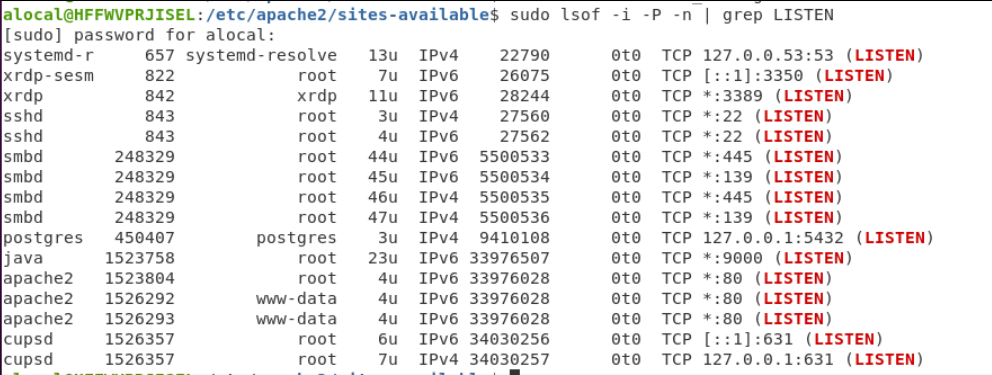
\includegraphics[scale=0.5]{Chapters/img/misc/ubuntu-services.png}
    \caption{Command to list currently listening processes.}
    \label{fig:list-programs}
\end{figure}



To host the application within the running Apache service, we need to create a configuration file made of Apache Directives tailored to the needs of the application. In conjunction to this file used by Apache it's also needed to enable the necessary modules for the configuration to work.
Firstly, the default location for the configurations of each web site hosted on Apache is in \lstinline[keywordstyle=\color{black},commentstyle=\color{black},stringstyle=\color{black}]{/etc/apache2/sites-available}, from there, we can create our custom configuration in a file created via the command line with \lstinline{sudo nano casciffo.conf}. 

The configuration consists in setting up a virtual host listening on port 80, the default port of HTTP, since the application is supposed to be available over HTTP. The term Virtual Host refers to the practice of running multiple web sites on a single machine. These web sites can be IP-based meaning that what differentiates each web sites is their IP-address, or, as in this case, name-based meaning that each web site has a different host name. 
The users of this application need a way of accessing it, as we're using a name-based approach, the name of the virtual host needs to be defined, this can be achieved with the properties \lstinline{ServerName} and \lstinline{ServerAlias}, which were both set to \lstinline{casciffo.hff.corp}. This allows the user to connect to the virtual host by navigating to the URL \lstinline[keywordstyle=\color{black},commentstyle=\color{black},stringstyle=\color{black}]{http://casciffo.hff.corp}, however it will currently only show the Apache web server default page.

To follow-up, to have the application be hosted the property \lstinline{DocumentRoot} is required to specify the location of the root directory of this virtual host, and as mentioned previously, the directory is \lstinline[keywordstyle=\color{black},commentstyle=\color{black},stringstyle=\color{black}]{/srv/casciffo}, which is the value of the property in question. 

Furthermore it is a best practice to include error and custom log files of the virtual host somewhere within the same directory, as such the properties \lstinline{ErrorLog} and \lstinline[keywordstyle=\color{black},commentstyle=\color{black},stringstyle=\color{black}]{CustomLog} 
were set to \lstinline[keywordstyle=\color{black},commentstyle=\color{black},stringstyle=\color{black}]{/srv/casciffo/error.log} and \lstinline[keywordstyle=\color{black},commentstyle=\color{black},stringstyle=\color{black}]{/srv/casciffo/custom.log}, respectively. The \lstinline{combined} keyword is a format used by Apache web that includes several pieces of information about each logged request.
This way we can perform monitoring operations on the application while being hosted and several other data analytics on the requests made.

Finally, although the user can reach the URL \lstinline[keywordstyle=\color{black},commentstyle=\color{black},stringstyle=\color{black}]{http://casciffo.hff.corp}, 
the application is not currently receiving any requests, to reroute the requests in order for the application to be able to respond to user requests we utilize the \lstinline{ProxyPass} and \lstinline{ProxyPassReverse} properties, which take in two argument, the first being the requested URL on the virtual host, followed by the target URL Apache web should proxy it towards. Since we want to proxy every request to the application, the first argument is set to \lstinline[keywordstyle=\color{black},commentstyle=\color{black},stringstyle=\color{black}]{/} while the target will be the URL of the running application.
Since the application is running on localhost and we know its port, the second argument is set to \lstinline[keywordstyle=\color{black},commentstyle=\color{black},stringstyle=\color{black}]{http://localhost:9000/}, as per our previous example on running the application indicated.

With the configurations set, we can proceed to the creation of the file \lstinline{casciffo.conf} as viewed in listing~\ref{lst:apache-conf}.
Having the configuration file created, all that's left is enabling the configuration through the command \lstinline{a2ensite casciffo} and reloading the Apache service with \lstinline{systemctl reload apache2}. However, doing this will result in an error due to the properties used, \lstinline{ProxyPass} and \lstinline{ProxyPassReverse} require the modules \lstinline{proxy} and \lstinline{proxy_http} both of which can be enabled with the command \lstinline{a2enmod}. With the purpose completing these commands, we can chain them and use the following command chain snippet:

\begin{itemize}
    \item \lstinline[keywordstyle=\color{black},commentstyle=\color{black},stringstyle=\color{black}]{sudo a2enmod proxy && sudo a2enmod proxy_http && sudo a2ensite casciffo.conf}
    \\ \lstinline[keywordstyle=\color{black},commentstyle=\color{black},stringstyle=\color{black}]{&& systemctl reload apache2}
\end{itemize}


\begin{lstlisting}[
caption={Apache configuration file.},
label={lst:apache-conf}
]
<VirtualHost *:80>
        ServerName casciffo.hff.corp
        ServerAlias casciffo.hff.corp

	DocumentRoot /srv/casciffo
	ErrorLog /srv/casciffo/error.log
	CustomLog /srv/casciffo/custom.log combined

        ProxyPass / http://localhost:9000/
        ProxyPassReverse / http://localhost:9000/
</VirtualHost>
\end{lstlisting}

Upon completing these steps, we can verify the correct functioning of the application through the virtual host, by accessing the site \lstinline[keywordstyle=\color{black},commentstyle=\color{black},stringstyle=\color{black}]{http://casciffo.hff.corp} from a different machine on the same network.